\documentclass[12pt,a4paper,twoside]{report}
\usepackage[utf8]{inputenc}
\usepackage[english]{babel}
\usepackage{indentfirst}
\usepackage{pdfpages}

\usepackage[titletoc]{appendix}

\usepackage{listings}
\usepackage{color}

\usepackage{graphicx}
\graphicspath{ {./images/} }

\usepackage{cite}
\usepackage{hyperref}
\hypersetup{
    colorlinks=true,
    linkcolor=blue,
    filecolor=magenta,      
    urlcolor=cyan,
}

\title{Bachelor's thesis}
\author{Tomáš Belluš}

\definecolor{codegreen}{rgb}{0,0.6,0}
\definecolor{codegray}{rgb}{0.5,0.5,0.5}
\definecolor{codepurple}{rgb}{0.58,0,0.82}
\definecolor{backcolor}{rgb}{0.95,0.95,0.95}
 
\lstdefinestyle{codestyle}{
    commentstyle=\color{blue},
    keywordstyle=\color{black},
    numberstyle=\tiny\color{codegray},
    stringstyle=\color{codepurple},
    showstringspaces=false,
    captionpos=b,
}
\lstset{style=codestyle}

\lstdefinestyle{appendix}{
    basicstyle=\small\ttfamily,
    showstringspaces=false,
    captionpos=b,
    numbers=left,
    stepnumber=1,
    numberstyle=\small,
    breaklines=true,
}

\newcommand{\myTitle}[0] {Network traffic capture and analysis}
\newcommand{\myName}[0] {Tomáš Belluš}
\newcommand{\mySupervisor}[0] {Ing. Dušan Bernát, PhD.}
\newcommand{\myEvidenceNumber}[0] {FIIT-104199-82385}
\newcommand{\myDate}[0] {May 2019}
\newcommand{\myStudyProgram}[0] {Internet Technologies}
\newcommand{\myStudyField}[0] {9.2.4 Computer Engineering}
\newcommand{\myFaculty}[0] {Faculty of Informatics and Information Technologies, FIIT STU, Bratislava}


\begin{document}

%title page
\begin{center}
\thispagestyle{empty}
{\Large Slovak University of Technology in Bratislava}
\par\end{center}{\Large \par}

\begin{center}
{\Large Faculty of Informatics and Information Technologies}
\par\end{center}{\Large \par}

\smallskip{}

\begin{center}
\myEvidenceNumber
\par\end{center}
\vfill{}

\begin{center}
\textbf{\Large \myName}
\par\end{center}{\Large \par}

\medskip{}


\begin{center}
\textbf{\LARGE \myTitle }
\par\end{center}{\huge \par}

\medskip{}


\begin{center}

{\Large Bachelor's thesis}
\par\end{center}{\Large \par}

\vfill{}


Supervisor: \mySupervisor

\medskip{}

\myDate

%assignment
\thispagestyle{empty}

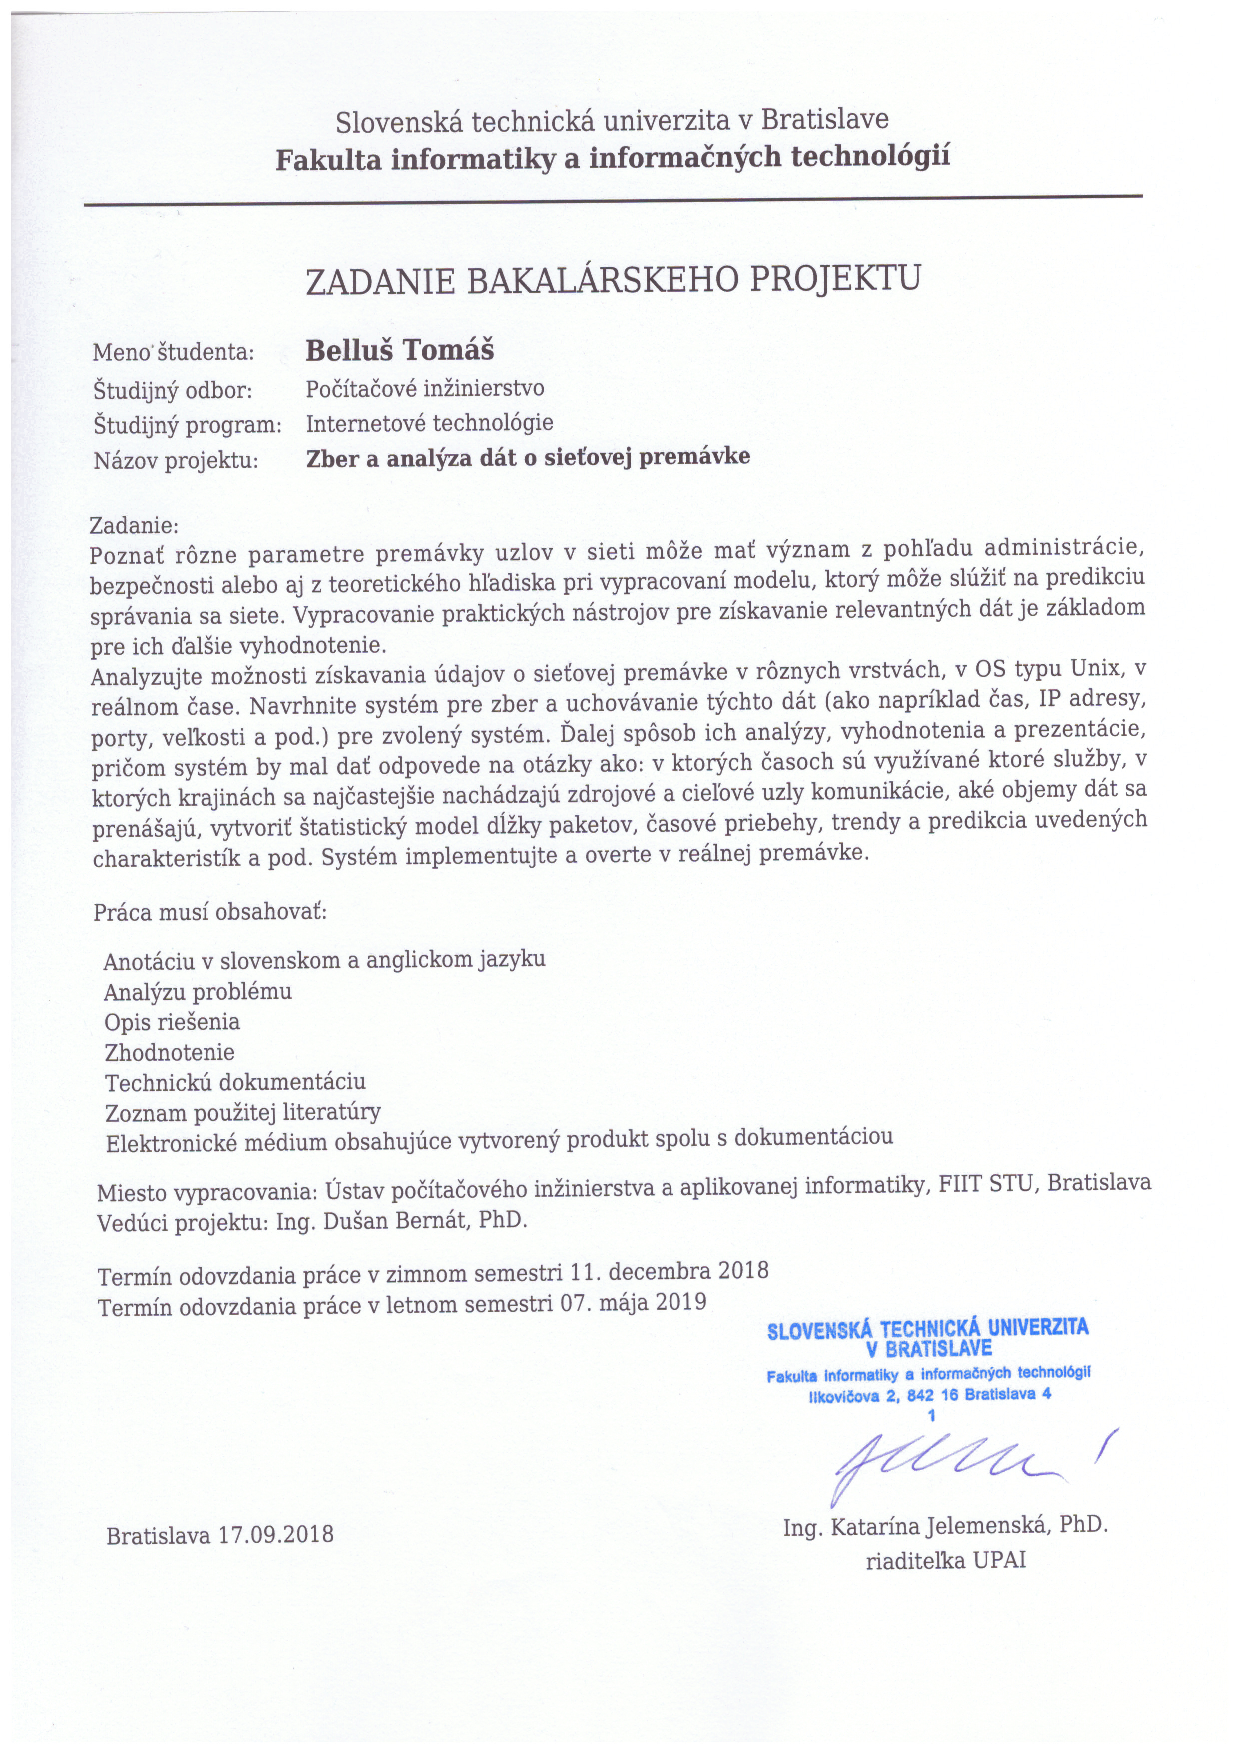
\includepdf[pages=-]{preamble/bp_zadanie.pdf}

\newpage{}\thispagestyle{empty}

\newpage
\thispagestyle{empty}
\mbox{}
\newpage

%declaration
\thispagestyle{empty}

\vspace*{\fill}
\begin{quote}
Hereby I declare that this bachelor's thesis was prepared as an original author's work under the supervision of \mySupervisor. All the relevant information sources, which were used during the  preparation of this thesis, are properly cited and included in the bibliography.\\

in Bratislava, \hfill signature\\
\begin{flushright}
......................\\
Tomáš Belluš
\end{flushright}
\end{quote}


\newpage{}\thispagestyle{empty}

\newpage
\thispagestyle{empty}
\mbox{}
\newpage

% annotation
%
\thispagestyle{empty}

\section*{Annotation}

\begin{minipage}[t]{1\columnwidth}%
Slovak University of Technology Bratislava 

Faculty of Informatics and Information Technologies

Degree Course: \myStudyProgram\\

Author: \myName

Diploma Thesis: \myTitle

Supervisor: \mySupervisor

\myDate%
\end{minipage}

\bigskip{}

\lipsum[3]


\newpage{}\thispagestyle{empty}

\newpage
\thispagestyle{empty}
\mbox{}
\newpage

\thispagestyle{empty}
\section*{Anotácia}

\begin{minipage}[t]{1\columnwidth}%
Slovenská technická univerzita v Bratislave

Fakulta informatiky a informačných technológií

Študijný program: \myStudyProgram\\

Autor: \myName

Diplomová práca: \myTitle

Vedúci diplomového projektu: \mySupervisor

\myDate%
\end{minipage}

\bigskip{}

\lipsum[3]


\newpage{}\thispagestyle{empty}\medskip{}


\newpage{}

\newpage
\thispagestyle{empty}
\mbox{}
\newpage

\newpage
\thispagestyle{empty}
{\center{Tu vložiť zadanie diplomovej práce}}
{\center{Potom, vložiť finálny návrh zadania diplomovej práce}}
\newpage


\thispagestyle{empty}
\mbox{}
\newpage



% acknowledgements
%include{preamble/acknowledgements}

% table of contents
\begingroup
\color{black}
\tableofcontents
\endgroup

\chapter{Introduction}
	Ever since the first two network devices, whether in telecommunications or computer networking, exchanged data in some manner, we began to urge ourselves to send, receive and analyze data. Sending and receiving for communicating, and analyzing for understanding. Nowadays, these concepts are very actual in network security, network statistics and network devices such as routers, switches, firewalls, servers or any end-point devices. Applications require fast packet capture mechanisms for further processing, to keep up with the world's ever-increasing trend of transfer rates.\par
	The Internet Protocol version 4 (IPv4) address range is, for a long time now, not enough for all devices connected to the largest network - the Internet. It implies that it is directly proportional to data being transfered over the Internet. This raises the need for applications, products or complex infrastructure solutions for keeping up with today's technologies. \par
	With increasing network transfers, number of network devices, new frameworks and transfer protocols, improved algorithms and overall network security comes the threat of data theft, (distributed) denial of service attacks, compromised system or network and many other. Therefore, real time network traffic analysis is of utmost importance for national security authorities (mainly cybernetic security department), security or network companies and even end-point users. Network traffic analysis includes understanding and depicting various indications of either unlawful actions for security reasons or network transfers for statistical purposes. For both it means monitoring the correct functionality of network at hand.\par
	Furthermore, each packet provides different decisive protocols that indicate information about the connection nodes and service used. A full understanding of the TCP/IP model and its layers is crucial for analyzing these services. Application, transport, network and link layer comprise the TCP/IP stack. Application layer is where applications exchange raw data, transport layer connects sockets for data transfer, network layer forwards packets to destination and link layer checks credibility and handles the closest physical device connections over medium.\par
	What are existing solutions to packet capturing mechanisms with network traffic analysis? How can we utilize existing packet capture mechanisms, reuse captured data analysis and identifying trends, threats and possibly predict future traffic? With packet capture and data analysis come storage systems, which need to be examined and evaluated. What known databases provide fast search process for real time network analysis and at the same time fast insertion rate, which would be sufficient for wire speed captures?\par
	This thesis aims to answer and evaluate these questions. In addition, consider frameworks, systems and mechanisms explicitly for UNIX systems. Implement a system for packet capturing, store captured data to chosen database and finally analyze it with a framework or tools. Create visualizations of how the network behaves, depict trends, make predictions of given characteristics and analyze network packets on different TCP/IP layers.\par
	\hyperref[analysis]{Chapter 2} analyzes packet capturing process, distinctions among various \hyperref[analysis:mechs]{mechanisms} in \hyperref[analysis:testing]{performance} and techniques, \hyperref[analysis:storage]{storage systems}, \hyperref[analysis:data]{data for analysis} and  \hyperref[analysis:solutions]{existing solutions}. \hyperref[solution]{Chapter 3} focuses on \hyperref[solution:spec]{system specifications}, \hyperref[solution:design]{system design} including the system architecture and \hyperref[solution:implementation]{implementation} including a data model.
\chapter{Analysis} \label{analysis}
	\section{Packet capture mechanisms} \label{analysis:mechs}
		The most critical part is real time data capture in network traffic, meaning capturing network packets using a framework or interpreted language library. It is a dependent process of hardware components like Network Interface Controller (NIC), processor performance and its properties (e.g. number of processor cores). Capture of every packet, which can be processed by arbitrary mechanism ordinarily takes place in the higher system layer - the user space. More efficient mechanisms have access to data, which fall under the jurisdiction of lower system layer - kernel space. Though, why is it more effective and efficient to access data in lower system layers? Kernel space is the operation system's (OS) core and an interface to hardware for the OS. More precisely, it is the access to shared kernel space, which altogether bypasses the additional copying and processing present with basic frameworks not utilizing efficient features.\par
		Received data on NIC is stored in NIC buffers. NIC registers keep track of whether the buffers are full and ready for reading or sending. This indication is handled by interrupts from the NIC to the OS. OS copies the buffer content to kernel space buffers (called \emph{m\_buffs} or \emph{sk\_buff}\footnote{These kernel buffers are expensive to create and vary in size. They are complex and include large amount of metadata. \cite{video:netmap}}). These buffers are not accessible by processes, but can be copied to user space or the process accessible memory. This is a typical scenario - two copies and interrupts needed for a process to access received data on the NIC. Possible improvements is to use, as mentioned above, buffers shared between kernel and user space, which eliminates one or more copies and interrupts from user to kernel space, leaving only one copy between NIC buffers and shared buffers. Other possibility is to have a NIC supporting multiple buffers, which split the load and each buffer is handled by different core simultaneously \cite{report:netmap}.\par
		A problem arises with the ability to capture all traffic on wire with no increasing delay resulting in packet loss due to lack of buffer space. Solution may be a zero-copy mechanism which utilizes a NIC dependent direct NIC access (DNA) or a one-copy mechanism, which utilizes the shared buffers. This section analyzes packet capture mechanisms, with various efficiency improvements at high packet rates in network traffic.
		\subsection{Scapy and RSS} \label{analysis:mechs:scapy_rss}
			\emph{Scapy}\footnote{\url{https://scapy.net/}} for Python running on Linux systems operates in user space with no access to shared memory. At its core it utlizes Libpcap library and it is mainly a packet crafting library, packet decoder and a network sniffing mechanism on given interface \cite{web:scapy}. In addition, it features filtering, detecting request responses and supports multiple existing protocols from all layers \cite{docs:scapy}. Even though, it has complex packet parsing, which makes it simple to extract any field, it is a huge bottleneck. It is present due to known Python complexity in lower layers of its implementation. While using scapy is a fast solution from development point of view, the execution time is crucial here, therefore its packet capturing performance is insufficient (see~\autoref{analysis:testing}).\par
			Additional resolution to the bottleneck, despite not using scapy, may be applying improvements to data processing on NIC driver level. It would require enabling CPU to process incoming packets by dividing received data among multiple CPU cores. On Linux platforms it is referred to as \emph{Receive-Side Scaling} \texttt{(RSS)} and it "distributes network receive processing across several hardware-based receive queues" \cite{web:redhat:rss}. More precisely, each queue will be handled by single core independently and simultaneously. Unfortunately, this feature is dependent of the NIC driver.
		\subsection{Packet socket} \label{analysis:mechs:socket}
			Creating a file descriptor \emph{packet socket}\footnote{\url{http://man7.org/linux/man-pages/man7/packet.7.html}} provides receiving and sending packets at datalink layer. It means that packets are captured before any processing in the Linux network stack as raw frames including all protocol headers \cite{man:packet}. A packet socket with raw network protocol access (raw socket) is opened by a system call (see~\autoref{lst:socket}), where the first argument must be \emph{AF\_PACKET}\footnote{AF\_PACKET is interchangable with PF\_PACKET and they stand for Address Family and Protocol Family respectively specified the communication domain.\cite{man:socket}} \cite{man:socket}, which indicates the protocal family. \emph{SOCK\_RAW} paramenter identifies that it is a raw socket providing a whole encapsulated Ethernet frame. Macro parameter \emph{ETH\_P\_ALL} specifies the socket protocol, which is expected on receive so in this case we require all protocols to be passed to socket interface \cite{man:packet}.
			\begin{lstlisting}[language=C, style=appendix, caption=Raw socket system call, label=lst:socket]
int fd = socket(AF_PACKET, SOCK_RAW, htons(ETH_P_ALL));
			\end{lstlisting}
			\par
			All in all, the packet socket is the interface receiving raw frames, or packets in case of trimming out link layer header, directly form the NIC and efficiently bypassing the network stack processing. This is an advantage concerning performance, because it produces only one copy of received data (from NIC driver to packet socket file descriptor) \cite{thesis:muni}\cite{web:raw_socket}. The shared memory between kernel and user space is the packet socket file descriptor. In contrast with basic address family \emph{AF\_INET}, packet socket provides socket option for packet capture statistics (PACKET\_STATISTICS), which is crucial for performance testing. In comparison with scapy it is the opposite in development and execution time point of view - it is presumably faster than scapy, but more complex to implement.\par
			\begin{figure}[h]
				\centering
				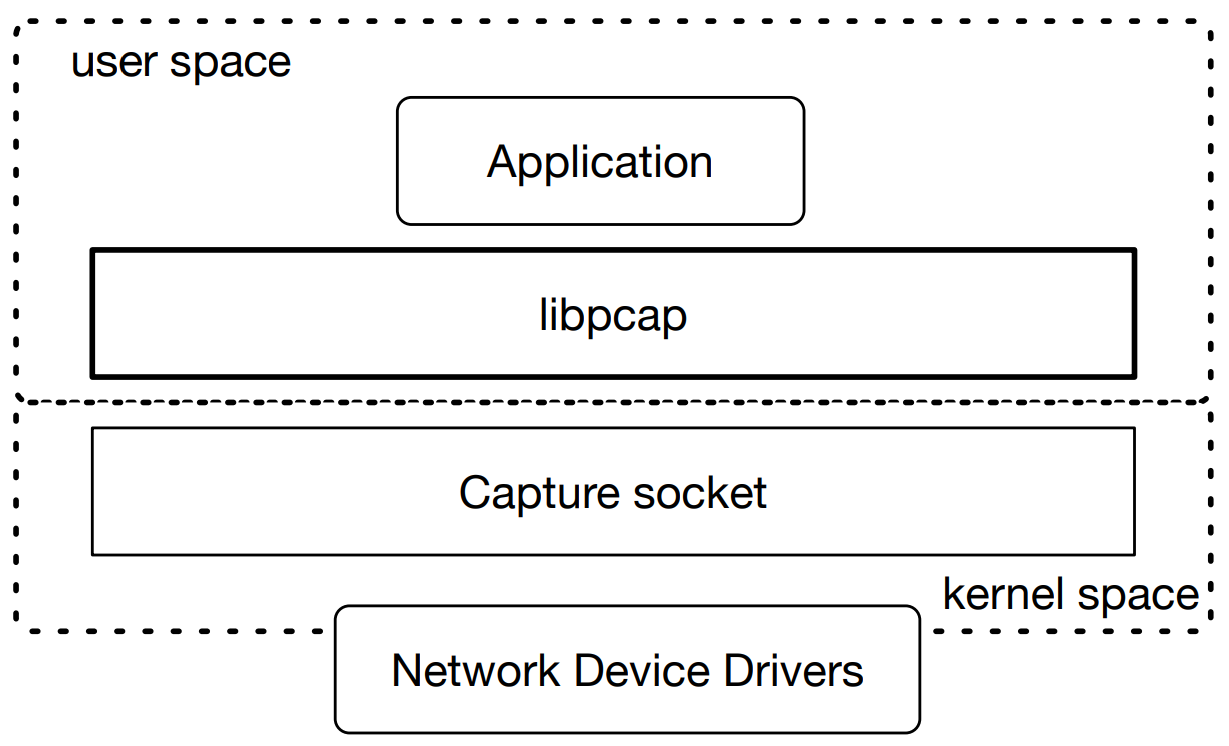
\includegraphics[scale=0.27]{linux_net_capture_struct}
				\caption{UNIX packet capture architecture for Libpcap or packet socket}
				\label{figure:libpcap:struct}
			\end{figure}
		\subsection{Libpcap} \label{analysis:mechs:libpcap}
			\emph{Libpcap}\footnote{\url{http://www.tcpdump.org/manpages/pcap.3pcap.html}} is an user space library designed mainly for capturing Ethernet frames. It is a cross platform library for UNIX systems not only for C/C++ programming (e.g \emph{tcpdump}\footnote{\url{http://www.tcpdump.org/manpages/tcpdump.1.html}} and \emph{wireshark}\footnote{\url{https://www.wireshark.org/}}), but for other more abstract languages (Python, C\#, Java, etc.) it exists in form of wrappers \cite{article:libpcap}. An user space library does not utilize kernel network stack, rather it reads raw Ethernet frames from opened socket queue in kernel space. Therefore, frame decapsulation is handled by libpcap and any protocol data, of parsed frame at hand, is accessed by libpcap's Application Programming Interface (API) (see~\autoref{figure:libpcap:struct}). Libpcap uses PF\_PACKET \cite{presentation:socket} \cite{report:libpcap} since version 0.6 release (year 2001) with kernel 2.2 support and later \cite{git:libpcap0.6:changes}.\par
			Moreover, as of libpcap release 0.9.5, this library supports capture statistics for protocol family PF\_PACKET by a \emph{getsockopt()} system call \cite{git:libpcap0.9:changes}. In reference to \hyperref[analysis:mechs:scapy_rss]{scapy} and \hyperref[analysis:mechs:socket]{packet socket}, libpcap provides more abstraction to implementations by wrapping socket operations to library functions and similar performance to packet socket.
		\subsection{PF\_RING} \label{analysis:mechs:pfring}
			Moving from user space library to the kernel space modules and possible zero-copy mechanisms, brings \emph{PF\_RING}\footnote{\url{https://www.ntop.org/products/packet-capture/pf_ring/}}. On socket layer it is a protocol family, replacing PF\_PACKET, but it requires loading a kernel module. On application layer, PF\_RING has an API for accessing received packets. PF\_RING lacking extra enhancements and independent of NIC driver is referred to as PF\_RING Vanilla. As of performance, through Linux New API (NAPI)\footnote{NAPI is a performance increase for packet capturing at higher packet rates, by enabling packet polling, therefore decreasing number of interrupts which otherwise would overwhelm the CPU \cite{web:linux:napi}} the kernel module copies polled packets from the NIC to shared memory ring buffers accessible by user application (see~\autoref{figure:pfring:overview})\cite{web:pfring:vanilla}. This process bypasses Linux network stack and the standard NIC driver. On the other hand, the performance depends on multiple hardware-based queues (\hyperref[analysis:mechs:scapy_rss]{RSS}) in form of shared memory ring buffers (see~\autoref{lst:rss}). Nevertheless, at least one shared memory ring buffer is created after loading the module to kernel. \cite{docs:pfring:vanilla}
			\begin{lstlisting}[language=bash, caption=Enabling RSS \cite{docs:pfring:rss}, label=lst:rss]
insmod driver_module.ko RSS=4,4
# enables 4 queues per interface (in this case two)
# the driver_module is the PF_RING enabled NIC driver
			\end{lstlisting}
			\par
			Worth mentioning is the PF\_RING\_ZC, which is a zero-copy alternative to PF\_RING Vanilla. It is strictly NIC driver dependent framework, which neglects NAPI, kernel modules and standard NIC driver to maximize efficiency by directly accessing NIC (DNA) (see~\autoref{figure:pfring:overview}). Inserting the correct PF\_RING-provided NIC driver enables an interface to be opened in zero-copy mode\footnote{Interface in the zero-copy mode has the "zc:" prefix (e.g. eth0 in zero-copy mode is accessed by zc:eth0). \cite{docs:pfring:zero}}. Any application can access packets through its API on 1-10 Gbit links at wire speed \cite{docs:pfring:zero}, if the kernel is bypassed. Otherwise the driver replaces the standard NIC driver and is faster compared to PF\_RING Vanilla \cite{web:pfring:zero}. Disadvantages are, that while accessing NIC in zero-copy mode, standard networking is on hold until the device at hand is closed \cite{web:pfring:zero} and due to bypassing kernel packet filtering is missing \cite{docs:pfring:zero}.\par
			Most valuable is the modified libpcap library\footnote{\url{https://github.com/ntop/PF_RING/tree/dev/userland/libpcap-1.8.1}} (pfring-libpcap) provided by the PF\_RING framework. Pfring-libpcap requires the PF\_RING module inserted and applications need to be recompiled with linking the new libpcap and specifically linking PF\_RING library (libpfring) \cite{docs:pfring:libpcap}. 
			\begin{figure}[h]
				\centering
				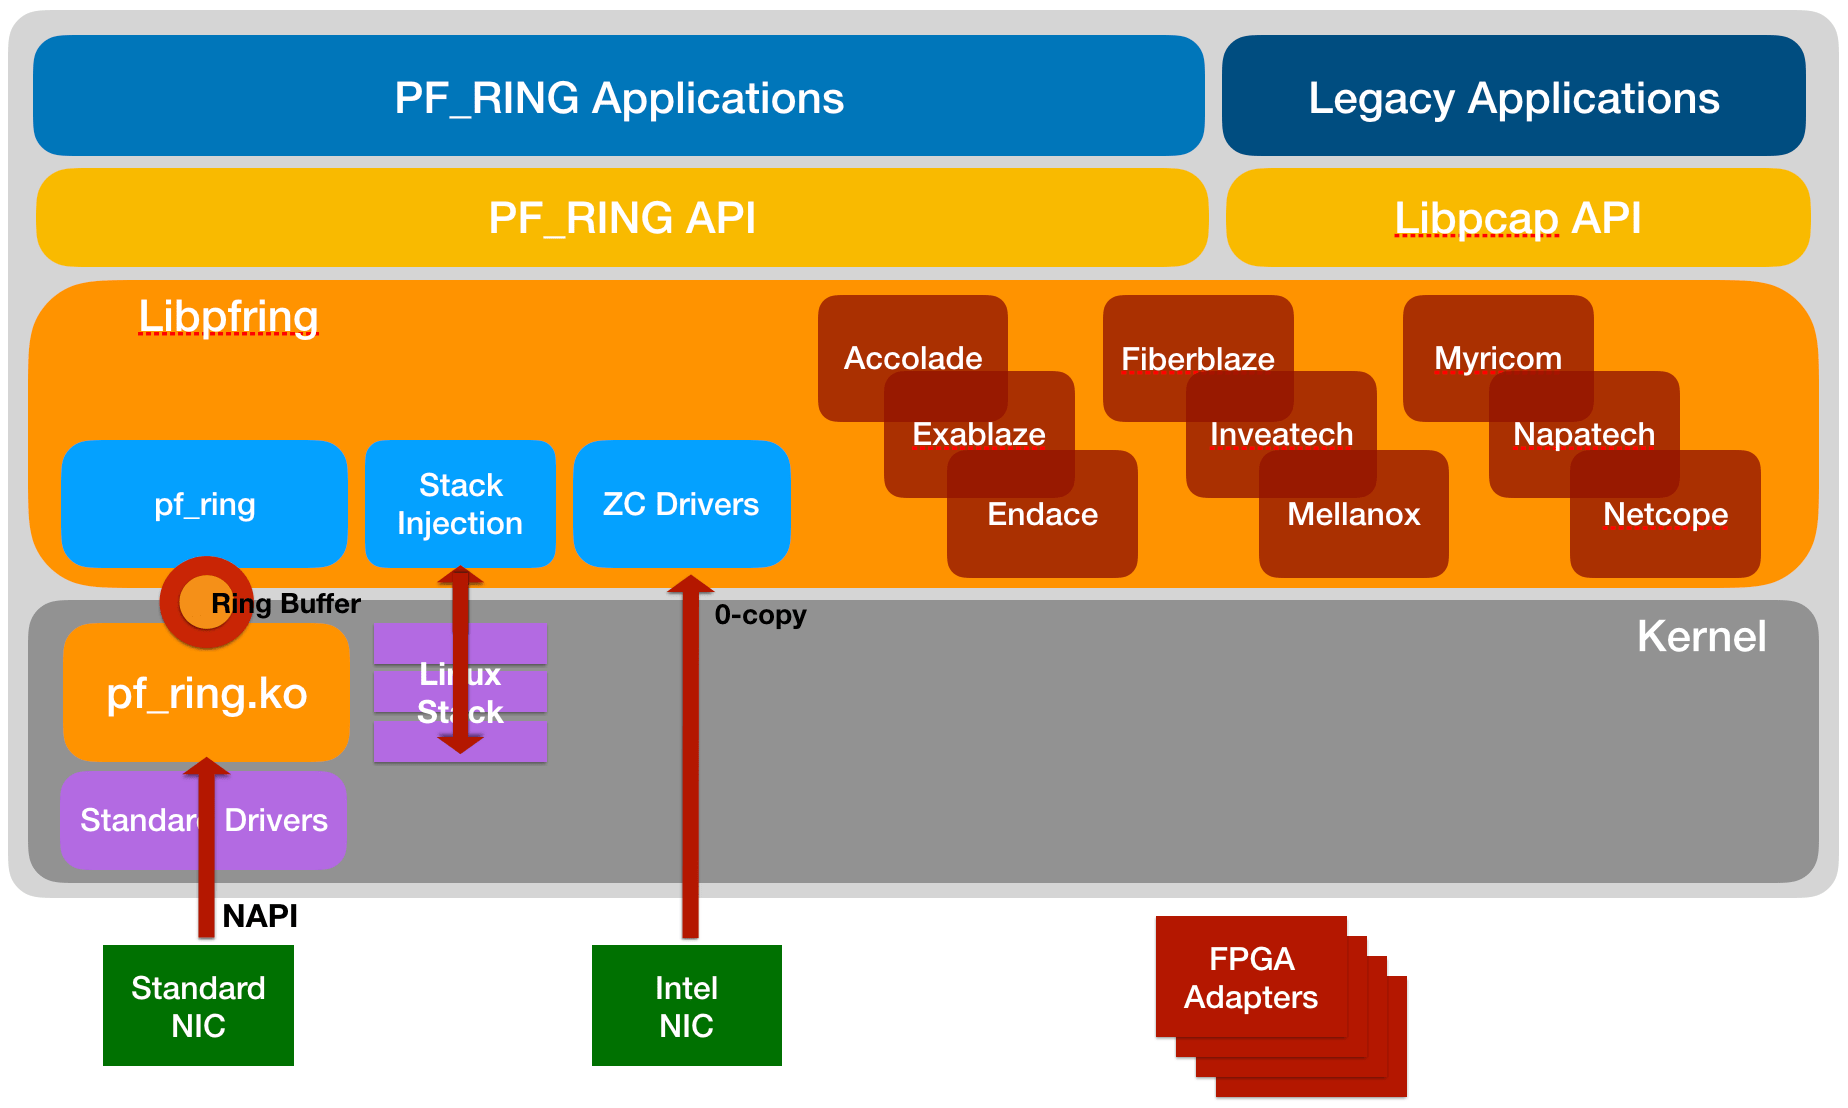
\includegraphics[scale=0.35]{overall_pf_ring}
				\caption{PF\_RING variants and architecture overview}
				\label{figure:pfring:overview}
			\end{figure}
		\subsection{Netmap} \label{analysis:mechs:netmap}
			Last, but not least capture mechanism with an API is \emph{netmap}\footnote{\url{http://info.iet.unipi.it/~luigi/netmap/}}. The current paragraph is derived from a report on Luigi Rizzo's netmap \cite{report:netmap}. "It is a framework to reduce the cost of moving traffic between hardware and the host stack" \cite{report:netmap}. Netmap targets the processing bottleneck by utilizing, similarly as PF\_RING or packet socket, the shared memory consisting of netmap packet buffers and netmap rings (buffer descriptors). The netmap packet buffers are shared between NIC rings and netmap rings, meaning that application processes access the packets in cost of one copy. In addition, the buffers are circular (ring buffers) and are designed (see~\autoref{figure:netmap:rings}) to eliminate most of the processing time. Standard NIC uses ring buffers for received data and the implementation of netmap rings is a replica of those buffers. The \emph{netmap\_if} is a descriptor table of netmap rings mainly used when multiple netmap rings are used for load balancing. In contrast with standard Linux packet capturing (I/O operations) process, where the buffers holding packets (\emph{sk\_buffs} or \emph{m\_buffs}) are allocated and deallocated throughout the capturing process, the netmap framework preallocates \emph{pkt\_bufs} (see~\autoref{figure:netmap:rings}) to bypass this time consuming operation.\par
			\begin{figure}
				\centering
				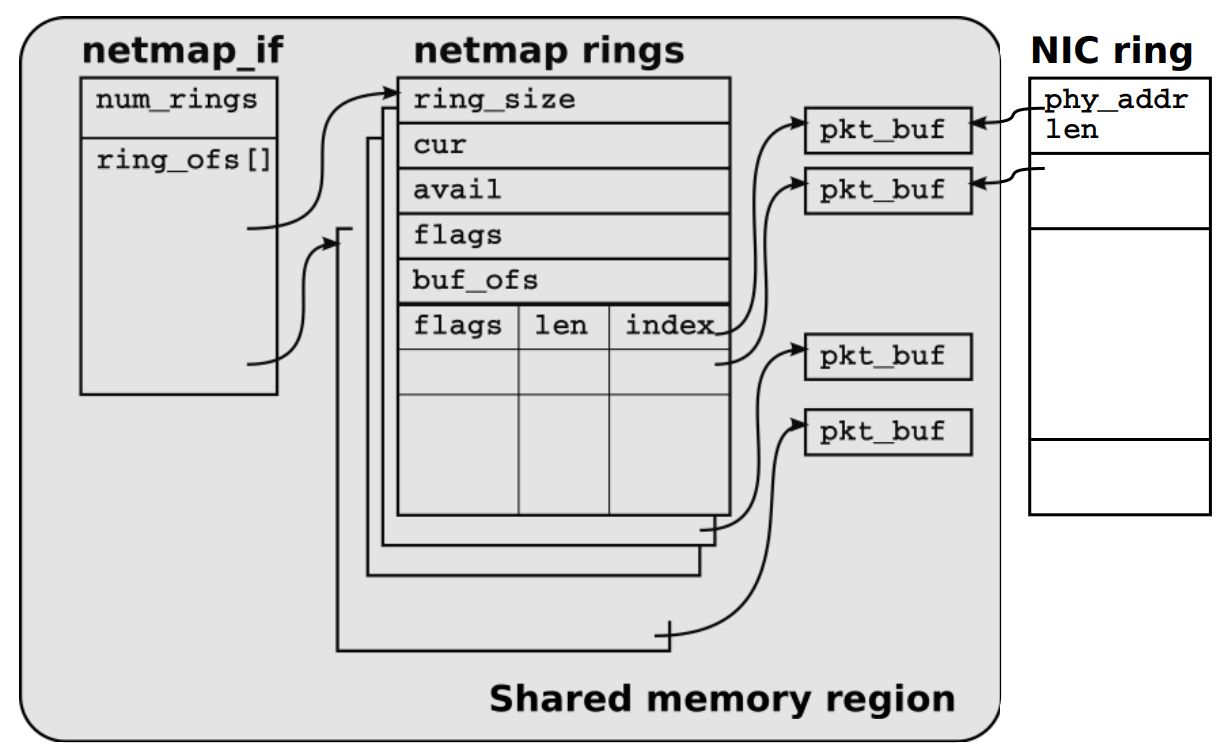
\includegraphics[scale=0.3]{netmap_rings}
				\caption{Netmap ring buffer design}
				\label{figure:netmap:rings}
			\end{figure}
			Moreover, it requires a modified driver to be loaded to kernel, which provides maximum performance at wire rate if the netmap native API is used. Just as PF\_RING, netmap provides a netmap-based libpcap by creating a modified library, which maps libpcap standard calls to netmap calls \cite{report:netmap}. Even though, the netmap libpcap has weaker performance in comparison with its native API, it does show improvement to the libpcap library \cite{video:netmap}. For compatibility purposes, opposing to the native API the netmap libpcap may be the most efficient mechanism variant.
	\section{Performance testing} \label{analysis:testing}
		All of the above are potentially effective packet capture mechanisms, but only few are efficient enough to produce expected results in reasonable time. Performance testing of any mechanism means to simulate expected network traffic environment and mark down elapsed time or other performance output based on specific mechanism. Requirements for efficient capturing mechanism are minimal or no packet drop rate combined with wire rate capture, bypassing kernel processing and minimizing data copies. Packet drop rate is the ratio of dropped packets and total packets received by a NIC during a given period of time. At wire rate capture, packets are received with no delay. Bypassing kernel altogether (except for handling interrupts) and minimizing data copies results in performance increase and it is a crucial mechanism feature. These are the three aspects for testing and comparing all \hyperref[analysis:mechs]{mechanisms} analyzed.\par
		This section focuses on performance testing process and its results. Packet capture efficiency (drop rate) of received traffic and time elapsed are measured and evaluated. Brief focus on \hyperref[analysis:testing:auto]{testing automation}, followed by the \hyperref[analysis:testing:tests]{specific tests} of both mentioned aspects and finally providing test \hyperref[analysis:testing:results]{results}.
		\subsection{Automation} \label{analysis:testing:auto}
			A bash script is used for efficient performance testing (see Appendices~\ref{appendix:script:droprate} and \ref{appendix:script:timed}) of both packet capture efficiency and elapsed time of captured traffic. For most mechanisms the implementation is straightforward, but running multiple executables (binary files) of single C program with various libpcap versions requires additional variables. It was the most crucial part of testing, since only one libpcap library version can be installed on a system. Appending the \emph{/etc/ld.so.conf} with directory paths of other libpcap versions partially solved the problem. Although, only one extra libpcap version can be added this way, since the linker works in a "first match" sense. For example, the target library was pfring-libpcap, but it was linked to netmap libpcap (see~\autoref{lst:compilation:pcap}).
			\begin{lstlisting}[language=bash, caption=Contents of /etc/ld.so.conf.d/libpcaps.conf, label=lst:compilation:pcap]
# paths to multiple libpcap libraries
/home/tomas/libpcaps/netmap-libpcap/
/home/tomas/libpcaps/PF_RING/userland/libpcap-1.8.1/
			\end{lstlisting}
			\par
			Solution is to link the library directly with the program source file, and on execution prefix the binary with overriding the LD\_LIBRARY\_PATH \cite{web:libraries:ldpath} environment variable (see Appendix~\ref{appendix:compilation:pcaps}). This variable may contain library paths to be searched before the library configuration file is used (\emph{/etc/ld.so.conf}). Setting the variable in line with execution makes it temporary, rather than sourcing it every other execution for different libpcap version. Using the \emph{ldd} command, which prints the shared object dependencies, validates this method a success.
		\subsection{Tests} \label{analysis:testing:tests}
			\begin{figure}[h]
				\centering
				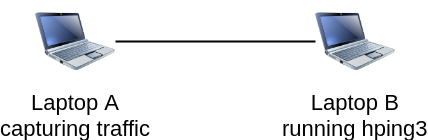
\includegraphics[scale=0.5]{diagram}
				\caption{Diagram of testing scenario}
				\label{figure:testing:diagram}
			\end{figure}
			\begin{table}[h!]
			\centering
			\begin{tabular}{ |p{2.0cm}||p{3.0cm}|p{1.3cm}|p{1.2cm}|p{3.0cm}| }
 				\hline
 				Machine & CPU & RAM & NIC & OS \\
 				\hline
 				Laptop A & Intel i5-7300HQ, 2.50GHz x4 & 16 GB & Realtek 1Gb & Ubuntu 18 64bit \\
 				\hline
 				Laptop B & Intel i5-2430M, 2,40Ghz x2 & 6 GB & Realtek 1Gb & Kali Linux 64bit \\
 				\hline
			\end{tabular}
			\caption{Computer hardware specifications}
			\label{table:pc_specs}
			\end{table}	
			Testing the packet capture efficiency required a traffic generator to simulate a high frequency of packets. For this purpose, Kali Linux has a generator tool \emph{hping3}, which is capable of sending 179 000 packets per second (179 Kpps) on a Realtek\footnote{RTL8111/8168/8411 PCI Express Gigabit Ethernet Controller} adapter. Even though, it is not a perfect real life traffic simulator it is sufficient enough to depict differences between some mechanisms. The testing environment consisted of two computers as shown in \autoref{figure:testing:diagram} with specifications in \autoref{table:pc_specs}. Drop rate is the best indicator of an efficient capture mechanism. Each test was constructed by the \emph{hping3} command generating raw IP packets with 120-byte payload at different frequencies (see Appendix~\ref{appendix:hping3}). Each mechanism was implemented as a simple C program or Python script and tested 5 times in 30 second time blocks. Refer to the Appendices for \hyperref[appendix:script:droprate]{bash script} for testing packet capture efficiency.\par		
			In contrast, testing capture elapsed time proves the wire speed capture of a mechanism. Similarly, \emph{hping3} tool was used for generating traffic at maximum rate (179 Kpps) using flood mode (see Appendix~\ref{appendix:hping3}). Each mechanism was tested 5 times with various number of packets to be captured subsequently returning elapsed time. Refer to the Appendices for \hyperref[appendix:script:timed]{bash script} testing elapsed time.\par
			In addition to this specific performance testing, a more precise and valuable tests were performed as part of the IIT.SRC 2019 conference included in Appendix \ref{appendix:iitsrc:paper}.
		\subsection{Results} \label{analysis:testing:results}
			Graphs displaying results of the performance tests are included in the Appendices \ref{appendix:tests:graph:drops}, \ref{appendix:tests:graph:timed} and \ref{appendix:iitsrc:paper}.
			\subsubsection*{Packet capture efficiency} \label{analysis:testing:results:capture}
				Results have proven that scapy is not effective at higher packet rates (see~\autoref{figure:tests:alldrops}), which is due to the Python complexity. It makes the drop rate increase rapidly, until more packets are dropped than captured (see~\autoref{table:scapy:drop}). Therefore, scapy is insufficient for capturing real time network traffic.
				\begin{table}[h]
					\centering
				\begin{tabular}{ |p{3cm}||p{3cm}|p{3cm}|p{3cm}| }
 					\hline
 					\multicolumn{4}{|c|}{Elapsed time test} \\
 					\hline
 					Packet rate [pkts/s] & received & captured & dropped \\
 					\hline
 					20	& 600 & 591 & 9 \\
 					194	& 5 820 & 5 726 & 94 \\
 					2 010	& 60 300 & 59 413 & 887 \\
 					20 050	& 601 500 & 87 711 & 513 789 \\
 					179 000	& 5 370 000 & 88 012 & 5 281 988 \\
 					\hline
				\end{tabular}
					\caption{Scapy measured drop rate}
					\label{table:scapy:drop}
				\end{table}
				\par
				Moreover, other mechanisms were efficient and captured all the traffic (no packets were dropped due to lack of buffer space). Referring to \autoref{figure:tests:closedrops}, packet socket is significantly faster at capturing packets at small rates, because it captures packets in a flow (one by one), rather than in batches\footnote{Capturing packets in batches means to copy or access multiple packets within one interrupt or read.}. As the rate increases, all mechanisms have zero drop rate and captured all packets. Deciding for a mechanism accords for potential zero-copy feature (netmap and PF\_RING), since all are equally efficient. Even though, netmap and PF\_RING could be compared as equally efficient, there are some major aspects analyzed in their respective sections, which breaks the tie.\par
				With respect to this test, netmap is the most suitable choice, because it provides minimum copies of data received, it has no measured drop rates and it is utilized in a modified netmap-based libpcap library, which makes the program compatible with other libpcap versions.
			\subsubsection*{Capture elapsed time} \label{analysis:testing:results:timed}
				Measuring the elapsed time of set of operations comprises of marking the time before and after the execution of target commands. This would be reliable if the system's time would not change due to Network Time Protocol (NTP) bad update or other unpredictable changes. Alternative is the monotonic clock, which goes forward independently of system's time. For Python scripts monotonic clock is included in \emph{time} module and for C it is included in \emph{time} library by \emph{clock\_gettime()}\footnote{\url{https://linux.die.net/man/3/clock_gettime}} system call.\par
				As it was for testing packet capture efficiency, elapsed time of packet capture with scapy was radically slow. As a result, scapy was not tested for the maximum of million packets because of the predicted exponential increase (see~\autoref{figure:tests:alltimed}). In comparison scapy was processing more than 30 seconds, while other mechanisms processed the same load in 500 ms. All other mechanisms captured packets in wire speed. \autoref{figure:tests:timed:best} compares average elapsed time for all considered mechanisms and netmap has processed million packets the shortest time. Even though, the bar graph shows differences between packet socket, netmap, PF\_RING and libpcap, their performance could be the same due to inconsistent packet rate on wire. Nevertheless, netmap did not fail this performance test, so it remains as the most efficient choice.
		\subsection{Summary} \label{analysis:mechs:final}
			There are multiple mechanisms considered and analyzed, but finally only netmap remained as the most efficient choice for both implementation and performance reasons. Therefore, netmap-based libpcap could be utilized for this thesis for compatibility and performance reasons.
	\section{Data storage} \label{analysis:storage}
		Initially, as it may seam, the most critical part is real time packet capture. Although, the real bottleneck in whole data processing is data storing in real time with acceptable time delay. Storing captured data includes parsing raw data and send them to a remote database server for further data analysis. This section analyzes considered database systems and options.
		\subsection{SQL versus NoSQL} \label{analysis:storage:sql}
			Using a Structured Query Language (SQL) database requires knowing the data model of the expected data - Relational Database Management System (RDBMS). This would require a complex data model of all possible fields of network protocols. SQL database stores full entries of data despite multiple empty fields, which produces extra disk space usage.\par
			However, Non-relational Structured Query Language (NoSQL) database provides high flexibility with its data and a faster search. Data can be stored in JSON format, which makes it directly compatible with numerous parsers and any data manipulation. NoSQL databases are also characterized as key-value pair database systems, such as Redis database, which is a simple caching database, MongoDB or Elasticsearch.
		\subsection{ELK stack} \label{analysis:storage:elastic}
			ELK stack\footnote{\url{https://www.elastic.co/elk-stack}} stands for \emph{Elasticsearch}, \emph{Logstash} and \emph{Kibana}, but at this point there are more possible components of the ELK stack (e.g. \emph{Filebeat}). The database component Elasticsearch, is a NoSQL database with no fixed data model. In comparison with a SQL database, where data is stored in records and tables, Elasticsearch stores data in documents and indices. Communication with an Elasticseach database is through various APIs using well known HTTP methods GET, POST, PUT and DELETE is in JSON query format.\par
			An Elasticsearch index is populated by documents in JSON format and is defined by its settings API and mapping API. Via settings, the default number of shards\footnote{Indices may be split into multiple sub-indices called shards.} and the number of replicas\footnote{Shard copies, functioning as a failover. The number of replicas represents the number of copies of each shard.} \cite{docs:elastic:terms} is defined. The mapping defines the document expected field's value type, but in case of lacking a concrete field mapping a document insertion does not fail.\par
			\begin{figure}
				\centering
				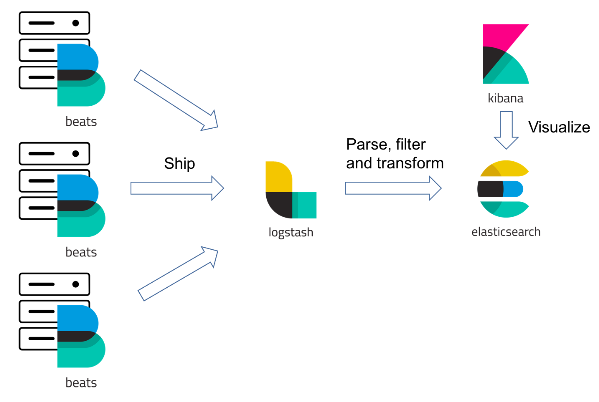
\includegraphics[scale=0.5]{logstash-filebeat}
				\caption{ELK stack set up including Filebeat}
				\label{figure:storage:elk}
			\end{figure}
			Logstash provides parsing, filtering and queuing data streams from multiple sources to be inserted into Elasticseacrh database (see~\autoref{figure:storage:elk}). It is useful for data enrichment and modification before it is inserted in bulk\footnote{Documents wrapped in batches sent via one HTTP request \cite{docs:elastic:bulk}.} requests, rather than single documents. In its configuration are data input streams' specifications, filter clauses including transformations and output stream, which is usually the Elasticsearch database. It reads various input streams like Filebeat, Elasticsearch or raw TCP data stream.\par
			In contrast, Filebeat is a lightweight component reading raw inputs, such as system log files or TCP raw data stream, which are redirected either directly to Elasticsearch or Logstash for more transformations and queuing purposes.\par
			Kibana is an optional component of the ELK stack capable of visualizing and monitoring data in Elasticseach (see~\autoref{figure:storage:elk}). It is an user friendly Elasticsearch interface, which abstracts the request queries when creating a visualization. For example, Kibana could serve as the Graphical User Interface (GUI) of the data stored in database for a network monitoring team of specialists. In addition, it recognizes a compatible timestamp formatted field for complex time period selections from any index or a specific data set. Moreover, to extend a field value, or creating a new field (visible only for Kibana) is possible by using scripted fields feature. All these features, creating visualizations or querying data in a NoSQL fashion are all advantages of using Kibana. Similarly as other ELK stack components, Kibana has a configuration file for specifying the ELasticsearch database.\par
			In comparison with a SQL database, Elasticsearch documents are populated with only provided fields, despite being defined in the mapping or not. Whereas, SQL database does always insert into all fields even if they are empty. This Elasticsearch advantage saves space and makes the search elastic and fast. Utilizing ELK stack would require an external system connected to the sensor, or it could be residing on the same physical machine.\par
		\subsection{Redis} \label{analysis:storage:redis}
			As an in-memory solution, where data analysis would take place as a part of the program and not as an external system connected to it, \emph{Redis}\footnote{\url{https://redis.io/}} could be the solution. Redis is widely used as a caching database \cite{docs:redis}, which would require analyzing and implementing the visualization of data as a part of the final program. In addition, the data received would not be stored, rather cached in Redis database.
		\subsection{Sumamry} \label{analysis:storage:conclusion}
			Since SQL databses are not suitable and Kibana provides the visualization tool for received data at arbitrary time period from the past, the ELK stack could be the right database system for this thesis.
	\section{Data visualization} \label{analysis:data}
		Data visualization will be done by the ELK stack component Kibana. It meets all visualization requirements, such as selecting a specific time period, creating bar graphs, heat maps or trend lines and updating all as new data is received. This section discusses the data worth visualizing for further analysis. We will consider all layers of the TCP/IP model - \hyperref[analysis:data:network]{Network layer}, \hyperref[analysis:data:transport]{Transport layer} and \hyperref[analysis:data:application]{Application layer}.
		\subsection{Network layer} \label{analysis:data:network}
			Collected data at this layer include endpoint nodes, source and destination IP address, nested protocol of the higher layer, the size of the packet at hand and the Time To Live (TTL) field. IP address is a valuable field, containing multiple properties of the endpoint. The IP address provides the location of the node, Autonomous System Number (ASN) of a specific Internet service provider, whether its an unicast, multicast or broadcast or it being a private or public IP address (regarding IPv4). Moreover, the Total length field (16-bit packet length) indicator can be used to detect large data transmissions. If the length is and very frequent, it could indicate unlawful activity or predict link failure for it would not withstand that high packet rate.\par
			\begin{figure}[h]
				\centering
				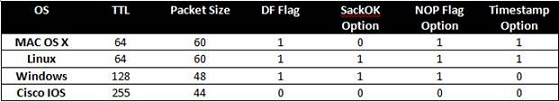
\includegraphics[scale=0.7]{osfingerprinting}
				\caption{OS fingerprinting with known IPv4 fields}
				\label{figure:data:osfinger}
			\end{figure}
			Additionally, according to an article on operating system (OS) fingerprinting with packets \cite{web:osfinger}, the TTL, packet size, flags and other option fields in the IPv4 protocol header can be used to determine the OS of the source endpoint (see~\autoref{figure:data:osfinger}). Based on this assumption, the network traffic is analyzed from more security concerned point of view, by grouping hosts by OS.
			Other frequent network layer protocol Internet Control Message Protocol (ICMP), as the name defines, is used in various network use-cases for notification purposes. For example, \emph{traceroute} protocol utilizes a property of a network device responding with an \emph{ICMP Time Exceeded} message, when the TTL counter reaches zero. ICMP is also used in routing protocols, such as RIPv2, and is most recognized as protocol utilized by \emph{ping} program used for debugging connectivity issues.
		\subsection{Transport layer} \label{analysis:data:transport}
			Transport layer provides more information on the communication, specifically port numbers, which identify the the service over which data is transmitted. Most recognizable Transport layer protocols are Transmission Control Protocol (\hyperref[analysis:data:transport:tcp]{TCP}) and User Datagram Protocol (\hyperref[analysis:data:transport:udp]{UDP}). TCP is used for services requiring reliable transmissions and do not require fast delivery, whereas UDP provides fast transmit rates at cost not being reliable.
			\subsubsection{TCP} \label{analysis:data:transport:tcp}
				Services like SSH, FTP, Telnet, HTTP(S), BGP, SMTP and more are transfered by the TCP protocol. TCP header includes the source and destination port numbers, where usually one is higher (client public port 49152 - 65535) and the other is lower (server designated port 0 - 1023). According to this, it is possible to monitor when a well known service is being used in the network or when two endpoints are communicating with public ports. There are various indicators considering port numbers and the client-server model.\par
				Furthermore, the TCP flags may be used to detected a session has opened or closed with the SYN and FIN flags respectively. When following the standardized three-way handshake, the SYN flag stands for synchronize and should indicate a session start. The FIN referring to final, finish or finalize indicates the session close. This is only a brief explanation and of course there are more TCP flagged packets to be sent in between.
			\subsubsection{UDP} \label{analysis:data:transport:udp}
				UDP is much simpler protocol with minimum header fields. It is the source and destination port numbers, length of corresponding UDP header with data and an optional checksum field. UDP is used by DNS, DHCP, TFTP, NTP and more services, which in comparison with TCP, provide fast file transfer service (e.g. TFTP) or generic service transparent for basic user (e.g. DNS, DHCP or NTP). Like all services, these have specific port numbers too, which can be read from packet capture even if the communication is encrypted\footnote{Communication is encrypted on the application layer.}. The UDP datagram length can be used for UDP datagram size histograms and statistics or detecting a high data transmission on the network.
		\subsection{Application layer} \label{analysis:data:application}
			Since most of network traffic on this layer is encrypted (e.g. SSH, HTTPS, etc.), there are minimum unencrypted protocols, which data could be analyzed or visualized. Unencrypted services include HTTP, Telnet over port 23, DNS, DHCP, FTP, TFTP and more. Raw data of these protocols could be used for deeper analysis.\par
			\subsubsection{Unencrypted and encrypted} \label{analysis:data:application:encr}
				In scope of this thesis, DNS packets may be the most valuable UDP-related application service for analysis. Detecting and monitoring a DNS communication has high security reasons. A possible amplification attack is realized by DNS packets.\par
				Furthermore, HTTP, FTP and TFTP are unencrypted data transmitting protocols, which could carry potentially valuable informations. For example HTTP protocol could be used as the insecure communication between client and web server, database or any API. Intercepting this traffic could provide statistics of successful or failed requests ergo connections. File transfers over TFTP or FTP discloses all data, which is part of the transmitted message. For statistical reasons, it is not beneficial to capture this data, but detecting these protocols indicates usage of insecure transmission.\par
				Others protocols (e.g. SSH and Telnet) are communication protocols acquiring connection with a host device for remote control. SSH is a secure communication protocol, which could be analyzed even when encrypted \cite{web:ssh}, but it is complicated. Nevertheless, the SSH communication is analyzed by detecting TCP protocol with source or destination port 22. In contrast, Telnet may be used for the same purposes as SSH, but it is not advised for it is an unencrypted communication channel. All sensitive data, such as user names, passwords or file system contents must be transmitted over to remote control terminal and thereby disclosing it all on the way.
	\section{Existing solutions} \label{analysis:solutions}
		Existing software solutions \hyperref[analysis:solutions:moloch]{Moloch}, \hyperref[analysis:solutions:wireshark]{Wireshark} and \hyperref[analysis:solutions:solarwinds]{SolarWinds} partially depict the problem at hand.
		\subsection{Wireshark} \label{analysis:solutions:wireshark}
			\emph{Wireshark}\footnote{\url{https://www.wireshark.org/}} is a tool using standard libpcap library used for live deep packet analysis, pcap file analysis and following connection streams. It includes protocol hierarchy statistics, I/O graph view of received packets per second, endpoint and network session statistics and complex filtering options. Wireshark understands multiple protocols, outputs live packet capture and parses packets in hierarchical manner. Wireshark does not provide the required data visualizations.
		\subsection{Moloch} \label{analysis:solutions:moloch}
			\emph{Moloch}\footnote{\url{https://molo.ch/}} is similar to wireshark in a way of reading pcap files and life network traffic. It utilizes Elasticseach cluster for fast search operations and captures data with PF\_RING module. Moloch provides network sessions statistics, unique value occurrence in sessions (SPI view or graph), network connections graph view of search results and Elasticsearch cluster and Moloch capture node statistics. Although, various visualizations of received data is not included.
		\subsection{SolarWinds} \label{analysis:solutions:solarwinds}
			Specifically \emph{SolarWinds Deep Packet Inspection and Analysis tool}\footnote{\url{https://bit.ly/2FUWBRn}}, processes each received packet, but summarizes the gathered information to protocol statistics and packet classifications. Includes network latency testing in network segment for troubleshooting purposes. Does not provide deeper packet analysis (e.g. various protocol header fields) or arbitrary visualizations of captured data.\par
\chapter{Problem solution} \label{solution}
	The solution to the analyzed components and merging it to one functioning system is described in the following chapter. The system specification, including its properties and use cases is outlined in \autoref{solution:spec}. The design of the solution and the overall system architecture is introduced in \autoref{solution:design}. The concrete implementation techniques and class model is described in \autoref{solution:implementation}.
	\section{System specification} \label{solution:spec}
		The final system must include the network sensor implanted in network for capturing packets and the ELK stack, which as the sensor is on a Linux machine. The sensor must then process and parse the received packets into a compatible JSON format for storing it to the database system via an API call.\par
		The key processes that need to be included are as follows. Choosing an interface as the source of received traffic and specifying the direction (outgoing, incoming or promiscuous mode), specifying the database destination with an IP address and a port and provide filters to be applied on received packets. Furthermore, it must notify the user with potential errors or successful tasks (such as initialization of the sensor) in standard log files in designated system directory. The packet capture and further processing must not create a bottleneck and be ideally processing at wire speed. The system must have control over used space in the database. In such cases, the system finalizes the received data with summarized data and clear the disk space.\par
		Considering the data visualization, various line graphs, bar graphs, heat maps and trend lines will be periodically updated as new data is received. These visualizations must be modifiable and it must be possible to create new visualizations. The final data set must include all desired protocol header fields and packet meta data such as, timestamp of the received packet, source host of the received data and source interface of that host. The database system should not delay the data stream. The requested visualizations are listed and briefly explained in \autoref{sol:design:elk:vis} part \emph{Visualizations and database setup}.
	\section{Design} \label{solution:design}
		\begin{figure}
			\centering
			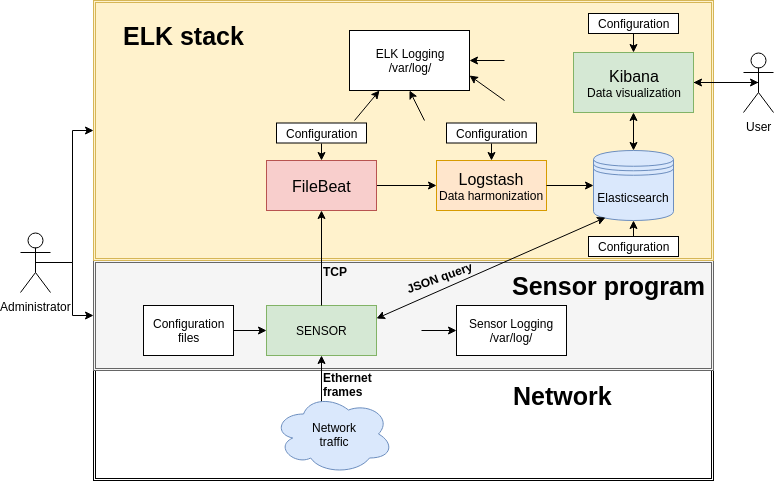
\includegraphics[scale=0.5]{architecture}
			\caption{System architecture model}
			\label{figure:sol:architecture}
		\end{figure}
		\subsection{ELK stack initialization} \label{solution:design:elk}
			Starting from the top of the system architecture model, the ELK stack setup is a prerequisite for functional sensor sending data to database. The deployment of the ELK stack on a remote or local server is handled by series of \emph{Ansible}\footnote{\url{https://www.ansible.com/}} roles. It will install each ELK stack component, including setting up required configuration files. Every component configuration is described in the following subsections. 
			\subsubsection*{Elasticsearch}
				Configuring Elasticserach requires setting up a new index for data and filling out the configuration file located in \emph{/etc/elasticsearch/elasticsearch.yml} (see~\autoref{lst:sol:elastic:conf}). After correctly configuring Elasticsearch, the index template is created via \emph{curl} program or via Kibana developer's tools (see~\autoref{lst:sol:mapping}).
				\lstinputlisting[language=Clean, style=appendix, label=lst:sol:mapping, caption=Create index template with index field mapping.]{src/create_template}
				The mapping of the index needs to include all fields. The proper way is to design it in a object form (e.g. \emph{source} object mapping in \autoref{lst:sol:mapping}). Mapping will correspond to real life data types, meaning an IP address has the type \emph{ip} or a geographical coordinates is of type \emph{geo\_point}. All mapping data types are listed in the Elasticsearch documentation\footnote{\url{https://www.elastic.co/guide/en/elasticsearch/reference/current/geo-point.html}}.
				\lstinputlisting[language=Clean, style=appendix, label=lst:sol:elastic:conf, caption=Elasticsearch configuration in YAML format]{src/elastic.conf}\par
				\emph{Path.logs} and \emph{path.data} specified the logging base directory and the path to archoved index data respectively. Most important is the \emph{network.host} in the example, which specifies that any remote system can access the database at specified port. This security vulnerability will be resolved by a firewall setting on the ELK stack server, allowing only the sensor host and localhost connections.
			\subsubsection*{Filebeat}
				Filebeat is configured with a host IP address and a port accepting TCP data. The JSON decoder in Filebeat is notified of receiving JSON formatted data via a tcp stream. All received data will be logged to corresponding log file. The output stream will be forwarded to Logstash socket specified by \emph{output.logstash.hosts} (see~\autoref{lst:sol:filebeat:conf}). In the background, filebeat harmonizes the data by filebeat specific fields. This example configuration sets a functional Filebeat receiving and forwarding JSON objects separated by \emph{new-line}.
				\lstinputlisting[language=Clean, style=appendix, label=lst:sol:filebeat:conf, caption=Filebeat configuration in YAML format]{src/filebeat.conf}
			\subsubsection*{Logstash}
				Refering the to the configuration (see Appendix~\autoref{appendix:implementation:logstash}), Logstash will be set up to listen on an arbitrary port and tagging the input. The filter clause removes undesired fields, and renames fields for data field misconception elimination. The original \emph{source} field holds the host address of the the source system sending data to Filebeat. The nested json clause creates a JSON object of the \emph{message} in JSON string type. Once the JSON object is created, the \emph{message} field may be deleted and a final field will be added to mark the future document with an identification of the filter clause used. The output clause sets the forwarding destination, which will be Elasticsearch database API, target index and document type.
			\subsubsection*{Kibana}
				Kibana is configured by a configuration file \emph{/etc/kibana/kibana.yml}. The default configuration (see~\autoref{lst:sol:kibana:conf}) from the installation is correct, since both Kibana and Elasticsearch will coexist on the same physical machine. The received data can be recognized and visualized by Kibana after setting up the index pattern and timestamp. New index pattern is created under Management \texttt{->} Kibana \texttt{->} Index Patterns only after the index occupies at least one document. This limitation can be bypassed by using the Kibana REST API.
				\lstinputlisting[language=Clean, style=appendix, label=lst:sol:kibana:conf, caption=Kibana sufficient default configuration]{src/kibana.conf}
			\subsubsection*{Visualization and database setup} \label{sol:design:elk:vis}
				With the index pattern set the requested visualizations are executed by Kibana on indices matching the index pattern. Each  visualization is periodically refreshed as new data is stored. Visualizations are grouped in dashboards (see Appendix~\ref{appendix:sol:dashboard}), which serves as the main page for further data analysis and monitoring. In addition, Kibana includes \emph{Developer tools} to request data with a JSON formatted query for fast search and the \emph{Discover} page which shows the latest received data. Other sections are not in scope of this thesis.\par
				Following the required visualizations, each is visualized by the most suitable representation:
				\begin{itemize}
					\item \emph{"Services in use"} are two line graphs (source and destination) displaying the count of packets based on the service (port number). Each line representing a service independent of transport protocol. The x-axis is the time at which the packets were captured. By filtering the services this visualization is for monitoring \emph{"specific service(s)"} too.
					\item \emph{"Geographical location of end nodes"} are two maps (source and destination of traffic) distinguishing multitude by color. The country is resolved from IP address either by the sensor or at the visualization tool.
					\item \emph{"Differentiating by IP protocol field"} displays UDP, TCP, ICMP and etc. protocol multitudes as a heat map, pie graph and line graph. Heat map groups by packet size ranges on one axis and protocol on the other. Pie graph depicting percentage ratio. Line graph specifically showing the multitude of protocols at a given time, where each line represents single protocol.
					\item \emph{"Statistical packet size model"} is a bar graph with time axis split by packet size ranges. The ranges specify the small packets, median sizes and large data packet sizes.
					\item \emph{"Packet flow"} is a line graph with time axis. Dots represent the total count of packets at particular time and a line representing the moving average of the values. It effectively shows the growth or descent of packet flow.
					\item \emph{"Visualization filters"} include the protocol filter, packet size range select, differentiating between receiving and transmitted (RX and TX) packets and service filter for destination and source port. This is not the filter limitation, but it depicts the most useful ones and other are possible.
					\item \emph{"Nodes' communications"} is a histogram or tag cloud displaying the most active connection between two hosts (IP addresses). 
				\end{itemize}
				
				To completely automate the initialization process and ready the visualizations all must be functioning when the visualization tool is opened. For Elasticsearch and Kibana it requires loading the index template, create visualizations, index patterns and dashboards. The reason for automation is if the system is duplicated or moved on different machines. It requires to preserve all settings, configurations and visualizations.\par
				Solution is to use Ansible for deploying the ELK stack components on the target machines. These Ansible roles deploy configured ELK stack components with functioning pipeline ready to receive data on Filebeat, which forwards them to Logstash and Elasticsearch. Missing are the visualizations, which need additional deploying mechanism to ready the visualizations and filters in Kibana. Kibana has its own REST API used for importing and exporting of saved objects\footnote{Saved objects include all index patterns, visualizations, dashboards and saved searches created in Kibana.}. \autoref{lst:sol:design:init_kibana} briefly depicts the necessary steps for initializing the Kibana environment.				
				\lstinputlisting[language=Clean, style=appendix, label=lst:sol:design:init_kibana, caption=Initialize Elasticsearch and Kibana.]{src/kibana_api}
				
		\subsection{Sensor} \label{solution:design:sensor}
			The sensor is a Linux program utilizing netmap-based libpcap (supported by \hyperref[analysis:testing:results]{test results}), the Kibana visualization tool and Elasticsearch as storage system. 
			\subsubsection*{Initialization}
				For sensor initialization, it requires
				\begin{itemize}
					\item a configuration file
					\item running \emph{rsyslog}\footnote{Rsyslog stands for rocket-fast syslog and it is the decedent of syslog.} server or syslog accepting local logs
					\item 
				\end{itemize}
				A suitable JSON library is used for parsing the packets to JSON structures, which are send to the ELK stack for storage and visualization (see~\autoref{figure:sol:architecture}). In between Kibana and the sensor, Filebeat accepts TCP data flow on an open port, specified by Filebeat configuration file. It represents the only communication channel between the sensor and ELK stack.\par
				Utilizing libpcap, the sensor captures traffic by simple receive, transmit or promiscuous mode and distinguish each packet by this indication. Each received packet is be parsed in scope of required protocols up to the Transport layer excluding the data payload (headers only). IP addresses are resolved in geological location database for country distinguishing. Parsed and harmonized packet data are converted to JSON objects. JSON objects are sent out as raw TCP data to Filebeat. Whole process is simplified in \autoref{figure:sensor:process}.
				\begin{figure}[h]
					\centering
					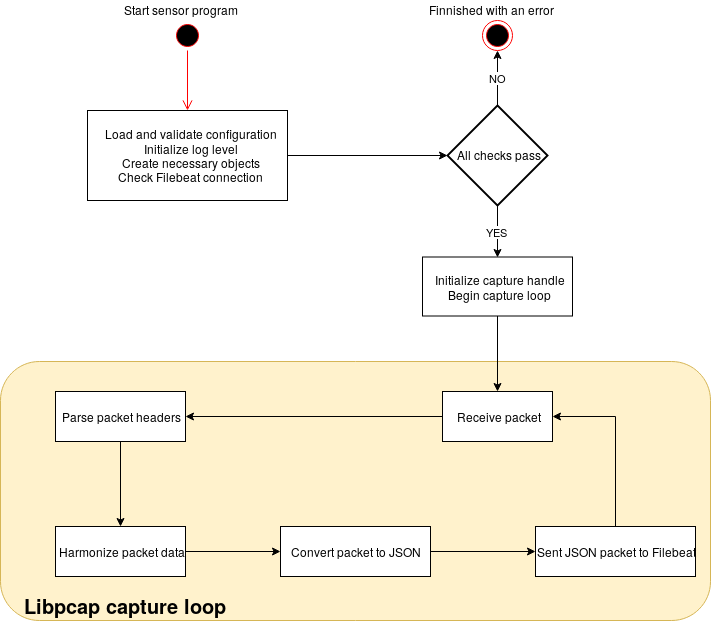
\includegraphics[scale=0.35]{sensor_process}
					\caption{Sensor packet parsing and processing}
					\label{figure:sensor:process}
				\end{figure}
			\subsubsection*{Data processing and storing} \label{solution:design:process}
				The sensor is configured by a configuration file, specified by the user. Both interface specification and filters will be included in this configuration file. Configuration file validation is, as other components logged to  success or error. Similarly, the capture will be logged on initialization and log error occurrence. For parsing packet structures, the most suitable library regarding conformance, parsing time, parsing memory and stringify time is \emph{RapidJSON}\footnote{\url{http://rapidjson.org/index.html}} \cite{git:benchmark:json}.\par
				Before any packet capture, an Elasticsearch index will be created with a given mapping in JSON format. Keeping consistent protocol field types, such as integers, strings or IP addresses is crucial to bypass Elasticsearch field recognization. Filebeat will accept TCP data flow on an open port and forward it to the Logstash service. Filebeat additionally appends some requested meta data, such as source host of the data and timestamp. Logstash has full control over this data and it will remove some extra meta data and add arbitrary static fields like overall data type identification (e.g. "sensor-data").\par
				The sensor will periodically monitor the database disk usage, until it detects low free space. In such case, the data will be summarized by multiple query requests and a new identical index will be created. Similarly, it will monitor the sensor log files and periodically archive large log files.
\chapter{Implementation} \label{solution:implementation}
	According to all specifications and speed requirements, the programming language will be C++, well compatible with netmap libpcap. The sensor will consist of a specific interface connection, packet parsing, logging and database connection. Referring to \autoref{figure:sol:architecture} the implemented component will be the sensor with external logging to files. The ELK stack is configured by respective configuration files and index creation via API call from Kibana developer tool or directly from remote host machine.
	\section{Sensor} \label{implementation:sensor}
		\begin{figure}
			\centering
			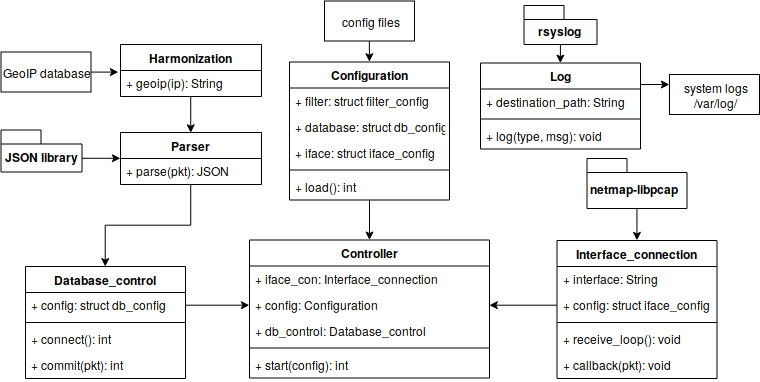
\includegraphics[scale=0.57]{datamodel}
			\caption{Class model of the implemented sensor}
			\label{figure:sol:datamodel}
		\end{figure}
		Sensor implementation requires efficient multi-threaded solution, where each component will be viewed as an object (see~\autoref{figure:sol:datamodel}). The main requirement - configuration file, will have a standard Linux white space separated format (e.g. \emph{/etc/hosts} file) with allowed bash style comments. The Configuration class loads the configuration file from the \emph{/etc/sensor/} directory to specific C++ structures - \emph{filter\_config, db\_configa, iface\_config} and validates the file's format. Components Interface\_connection and Database\_control are created with corresponding configuration structures, which contents are verified by connection attempt to database system, opening given interface file descriptor with specified filters. If any errors occur the message is logged and process terminated.
		\subsection{Configuration file} \label{implementation:sensor:config}
			Configuration file must be located in the designated directory for program configurations (\emph{/etc/sensor/conf.d/test.conf}). The main configuration file \emph{/etc/sensor/sensor.conf} will hold path to configuration files (see~\autoref{lst:config:main}).
			\begin{lstlisting}[language=bash, style=appendix, caption=Contents of main configuration file, label=lst:config:main]
/etc/sensor/conf.d/*.conf
			\end{lstlisting}				
			The configuration will be loaded on sensor startup and each line is loaded to corresponding data structure. Validations of configuration file will be logged to specific sensor log file. The configuration file must include the following fields. The source interface name must correspond to the name listed by \emph{ip link} or \emph{ifconfig} commands. The possible capture direction modes are "out" for outgoing packets, "in" for incoming packets and "promisc" for promiscuous mode. Packet capture filters are not compulsory, because they slow down the capture process. Nevertheless the allowed syntax is specified by the Berkeley Packet Filter syntax\footnote{\url{https://docs.extrahop.com/7.2/bpf-syntax/}}. The Filebeat and Elasticsearch connection specification must be a resolvable host IP address or host name and port must be a numbering ranging 0-65535. Archive path, must be an existing path on the local file system, where all summarized data will be archived. Archivation is limited by the \emph{archive\_limit} specified in mega bytes, when the index will be archived and cleared. \par
			In case of missing component, the system will log it as an error and request correction. For sample configuration and default configuration refer to the \autoref{lst:sensor:config} in the Appendices section.
		\subsection{Packet capturing} \label{implementation:sensor:cap}
			Netmap does not change the modified libpcap from programmers point of view. Packet capturing implementation consists of opening a file descriptor, applying filters to each received packet and opening a loop capture session (see~\autoref{lst:implementation:pcap}). After initialization of the \emph{Interface\_connection} class, the main packet receiving method will be a running thread in the \emph{Controller} class.
			\lstinputlisting[language=C++, style=appendix, label=lst:implementation:pcap, caption=Libpcap capture code sample]{src/pcap}\par
			All packet capture relying data is provided by the configuration file specifying the interface used, capture direction and filters.
		\subsection{Packet parsing} \label{implementation:sensor:parse}
			\emph{RapidJSON} library provides the \emph{Simple API for XML} (SAX API), which includes a JSON generator \emph{Writer}. Writer converts keys and values into JSON in a procedural manner (see~\autoref{lst:implementation:parsing}). The parsing is part of \emph{Parser} class and its main parse function takes a libpcap packet structure provided by the caller (\emph{Database\_control} class). Keys specified in the output JSON must correspond to the Elasticsearch database mapping field names. Parsing is expected to execute without errors, since the input is a libpcap packet structure and the output is a JSON string.
			\lstinputlisting[language=C++, style=appendix, label=lst:implementation:parsing, caption=Packet parsing to JSON format]{src/parsing}
		\subsection{Committing packets to ELK stack} \label{implementation:sensor:commit}
			Connecting to the database system is part of the \emph{Database\_control} class. The connection parameters, including the Filebeat public IP address and the target port, are specified in a configuration file (see~\autoref{lst:sensor:config}). The established connection with the ELK stack component Filebeat, will provide a TCP stream of raw JSON data. Committing is expected to fail if the connection with Filebeat is lost, which will be properly logged. Successful commit will not be logged, because of the high frequency of commits. Sending data to Filebeat needs to be as fast as it was received and it will require another live libpcap session to send raw TCP data packets. The \emph{Parser} class provides the JSON data of the received packet to the \emph{Database\_control} class.\par
			This class receives packet structures from the packet capturing thread, running in the \emph{Controller} class, which has a running thread of committing packets to the database system. That is the multi-threaded part of the sensor.
		\subsection{Checking disk usage} \label{implementation:sensor:disk}		
			In a separate thread, running in the \emph{Controller} class, the \emph{Database\_control} class has a function monitoring the disk usage directly on the Elasticsearch node, whose connection specifications are read from the configuration structure. It will log the current database state (number of documents and disk usage) and check for low free space.
			\begin{lstlisting}[language=Clean, caption=Get number of documents and disk usage, label=lst:apicall:diskusage]
GET "elastic.bp:9200/_cat/shards?v"
[Sample output]
index   shard rep state   docs  store   ip       node
bp_test 2     r   STARTED 76661 415.6mb 10.0.0.1 Andromeda
			\end{lstlisting}				
			When the free space gets low, specifically under a specified limit, a periodic function (see simplified code sample in \autoref{lst:sol:checkusage}) checks for such scenario and executes specific tasks.
			\lstinputlisting[language=C++, style=appendix, caption=Simplified \emph{check\_disk} function, label=lst:sol:checkusage]{src/check_usage}
			Provided requests can be modified or created as a valid JSON formatted Elasticsearch GET API request query. The main configuration file \emph{/etc/sensor/requests.conf} will hold path to request files (see~\autoref{lst:config:requests}). 
			\begin{lstlisting}[language=bash, style=appendix, caption=Contents of main requests configuration file, label=lst:config:requests]
/etc/sensor/requests.d/*.conf
			\end{lstlisting}				
			The validity of GET requests is checked by Elasticsearch and received errors are logged. Additional GET requests must be tested on Elasticsearch beforehand, because there will be no warnings, besides the logs.\par
			Deleting documents by query, queries the index and removes all matched documents. The deleted portion of index frees up space without interfering with frequent data storing. The summarized data in request responses will be stored in the archive path in parsed structure (parsing JSON to readable data using \emph{Parser} class). According to the \hyperref[figure:sol:datamodel]{class model}, the \emph{understand} function returns a Document Object Model (DOM) object, which is a JSON parsed to C++ compatible object. Each archive file name will comprise of a timestamp and brief contents description distinguishing all archives.
			
			THIS BELONG TO KIBANA SETUP IMPLEMENTATION SECTION
			\lstinputlisting[language=Clean, style=appendix, label=lst:sol:init_kibana, caption=Initialize Elasticsearch and Kibana custom prerequisites.]{src/initialize_kibana}			
			
		\subsection{Logging} \label{implementation:sensor:logging}
			Logging to \emph{/var/log/sesnor/} directory will be handled by the \emph{Log} class. Logs will be structured including the event's timestamp, log message level, log's source and the raw message (see \emph{log} function in \autoref{figure:sol:datamodel}). The timestamp will be marked in the \emph{Log} class and other parameters will be passed by the caller object. Message level will be statically listed in the \emph{Log} class as an enumeration. For scalability purposes, each class utilizing logging will have a custom source identifier distinguishing it in the log file.\par				
			The existing message levels are infromative, warnings, errors or debugs.\emph{INFO\_LOG} notifies successful operations or messages of informative manner. \emph{WARN\_LOG} includes warning messages, which are avoidable, but a fix is advised. \emph{ERROR\_LOG} message often comprises of the exception message caught at sensor start up and object initializations. \emph{DEBBUG\_LOG} describes an optional output in the log file.\par
			Since, multiple sources will log to the same file, the \emph{Log} class has a \emph{mutex} lock object to handle mutual exclusion of the shared log file. On sensor start up or every 24 hours the log file size will be checked (see~\autoref{lst:sol:checklog}). If the size exceeds 10 MB, it will be archived in the same directory and compressed using the \emph{gunzip}\footnote{\url{https://www.gzip.org/}} compression tool by an OS system call (log rotation). The \emph{check\_log} function will be running in a thread under the \emph{Controller} class.
			\lstinputlisting[language=C++, style=appendix, caption=Simplified \emph{check\_log} function, label=lst:sol:checklog]{src/check_log}
	

\newpage
\bibliographystyle{plain}
\bibliography{sources}

\begin{appendices}
	\chapter{Bash script for drop rate} \label{appendix:script:droprate}
		\lstinputlisting[language=bash, style=appendix, label=listing:script:droprate]{src/script-droprate}
	\chapter{Bash script for elapsed time} \label{appendix:script:timed}
		\lstinputlisting[language=bash, style=appendix, label=listing:script:timed]{src/script-timed}
	\chapter{Linking various libpcap versions to one C source} \label{appendix:compilation:pcaps}
		\lstinputlisting[language=Clean, style=appendix, label=listing:compilation:pcaps]{src/compilation-proof}
	\chapter{Hping3 traffic generator} \label{appendix:hping3}
		\lstinputlisting[language=Clean, style=appendix, label=listing:hping3]{src/hping3_generator}
	\chapter{Packet capture graphs} \label{appendix:tests:graph:drops}
		\begin{figure}[h]
			\centering
			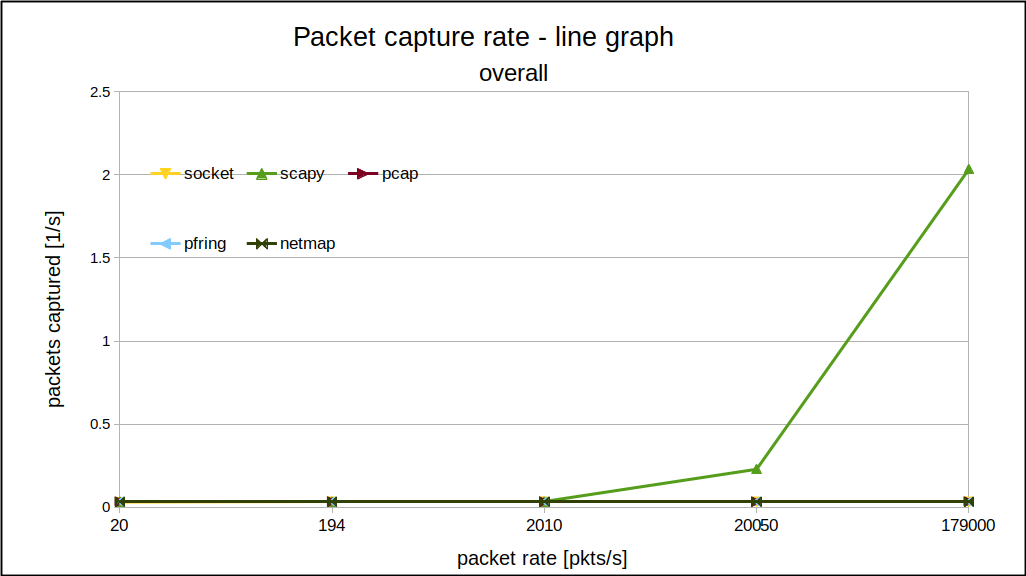
\includegraphics[scale=0.5]{overall_drops_line-graph}
			\caption{Capture performance for testing drop rate}
			\label{figure:tests:alldrops}
		\end{figure}
		\begin{figure}[h]
			\centering
			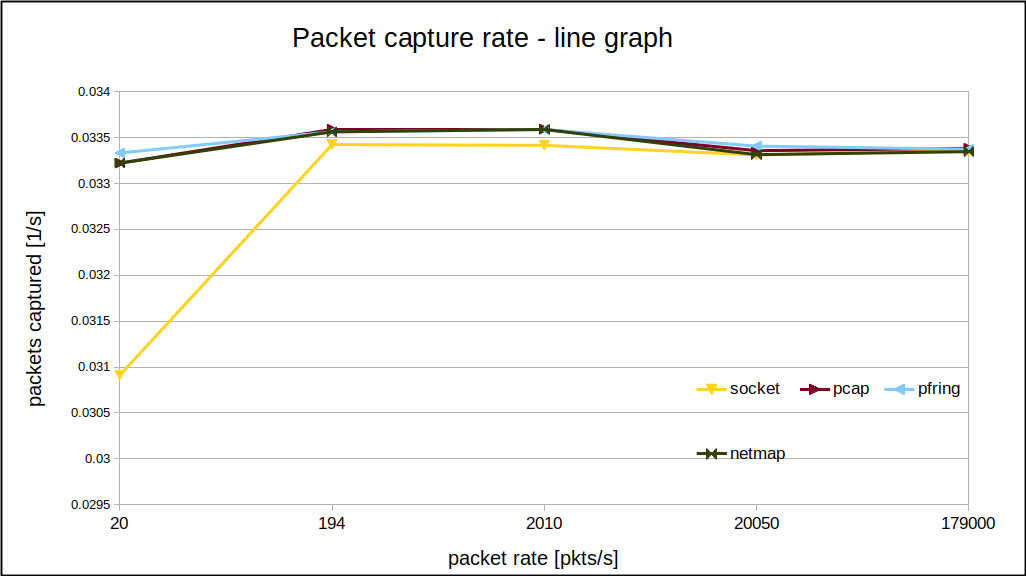
\includegraphics[scale=0.5]{closeup_drops_line-graph}
			\caption{Capture performance for testing drop rate. Number of packets captured in a second}
			\label{figure:tests:closedrops}
		\end{figure}
	\chapter{Packet capture elapsed time} \label{appendix:tests:graph:timed}
		\begin{figure}[h]
			\centering
			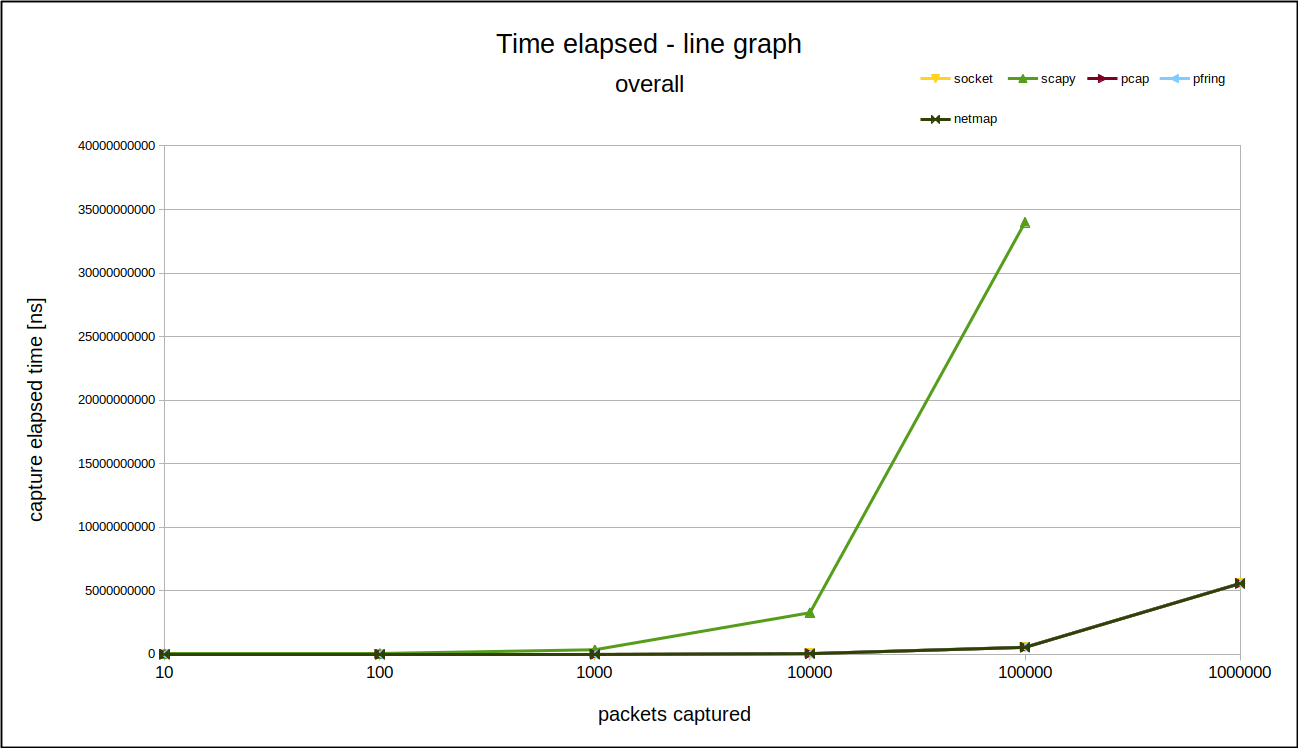
\includegraphics[scale=0.39]{overall_speed_line-graph}
			\caption{Capture performance for testing elapsed time}
			\label{figure:tests:alltimed}
		\end{figure}
		\begin{figure}[h]
			\centering
			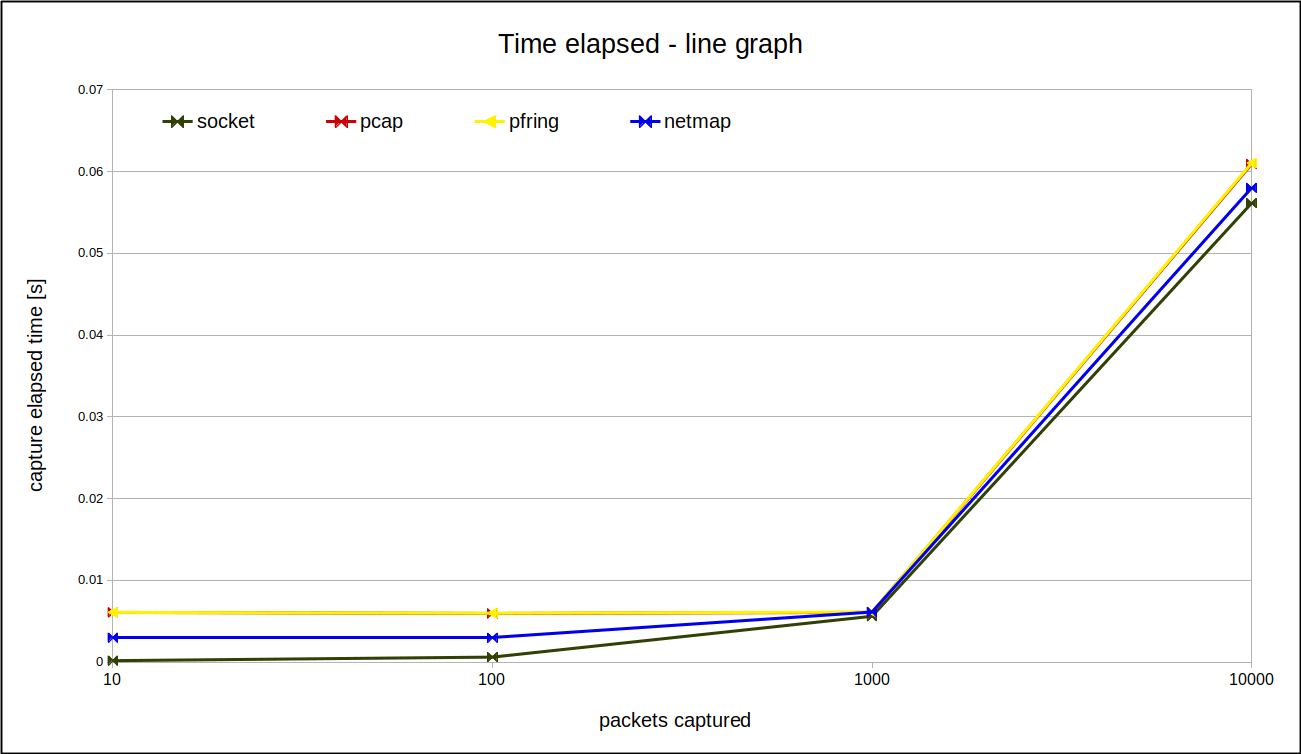
\includegraphics[scale=0.39]{closeup_speed_line-graph}
			\caption{Close up graph of capture performance for testing elapsed time and discarding scapy.}
			\label{figure:tests:closetimed}
		\end{figure}
		\begin{figure}[h]
			\centering
			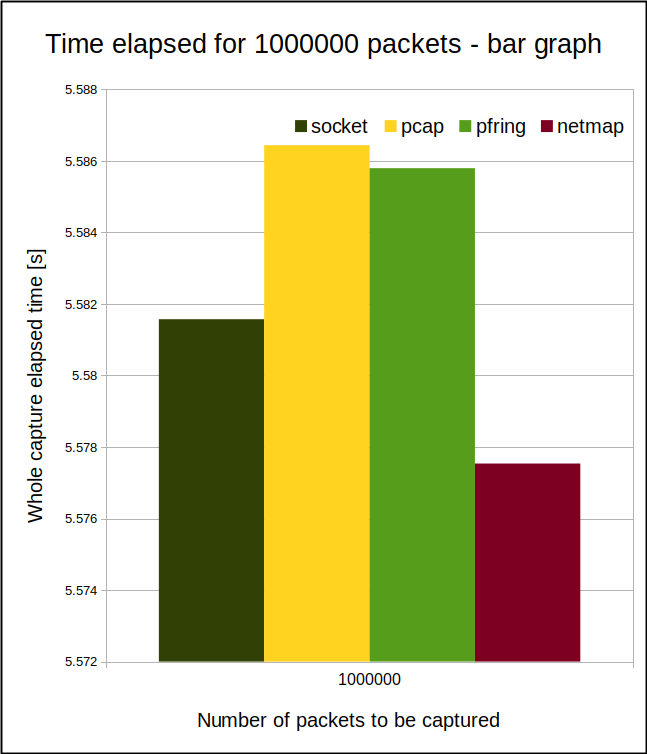
\includegraphics[scale=0.5]{speed_bar-graph}
			\caption{Best performance at million sent packets}
			\label{figure:tests:timed:best}
		\end{figure}
	\chapter{IIT.SRC research paper} \label{appendix:iitsrc:paper}
		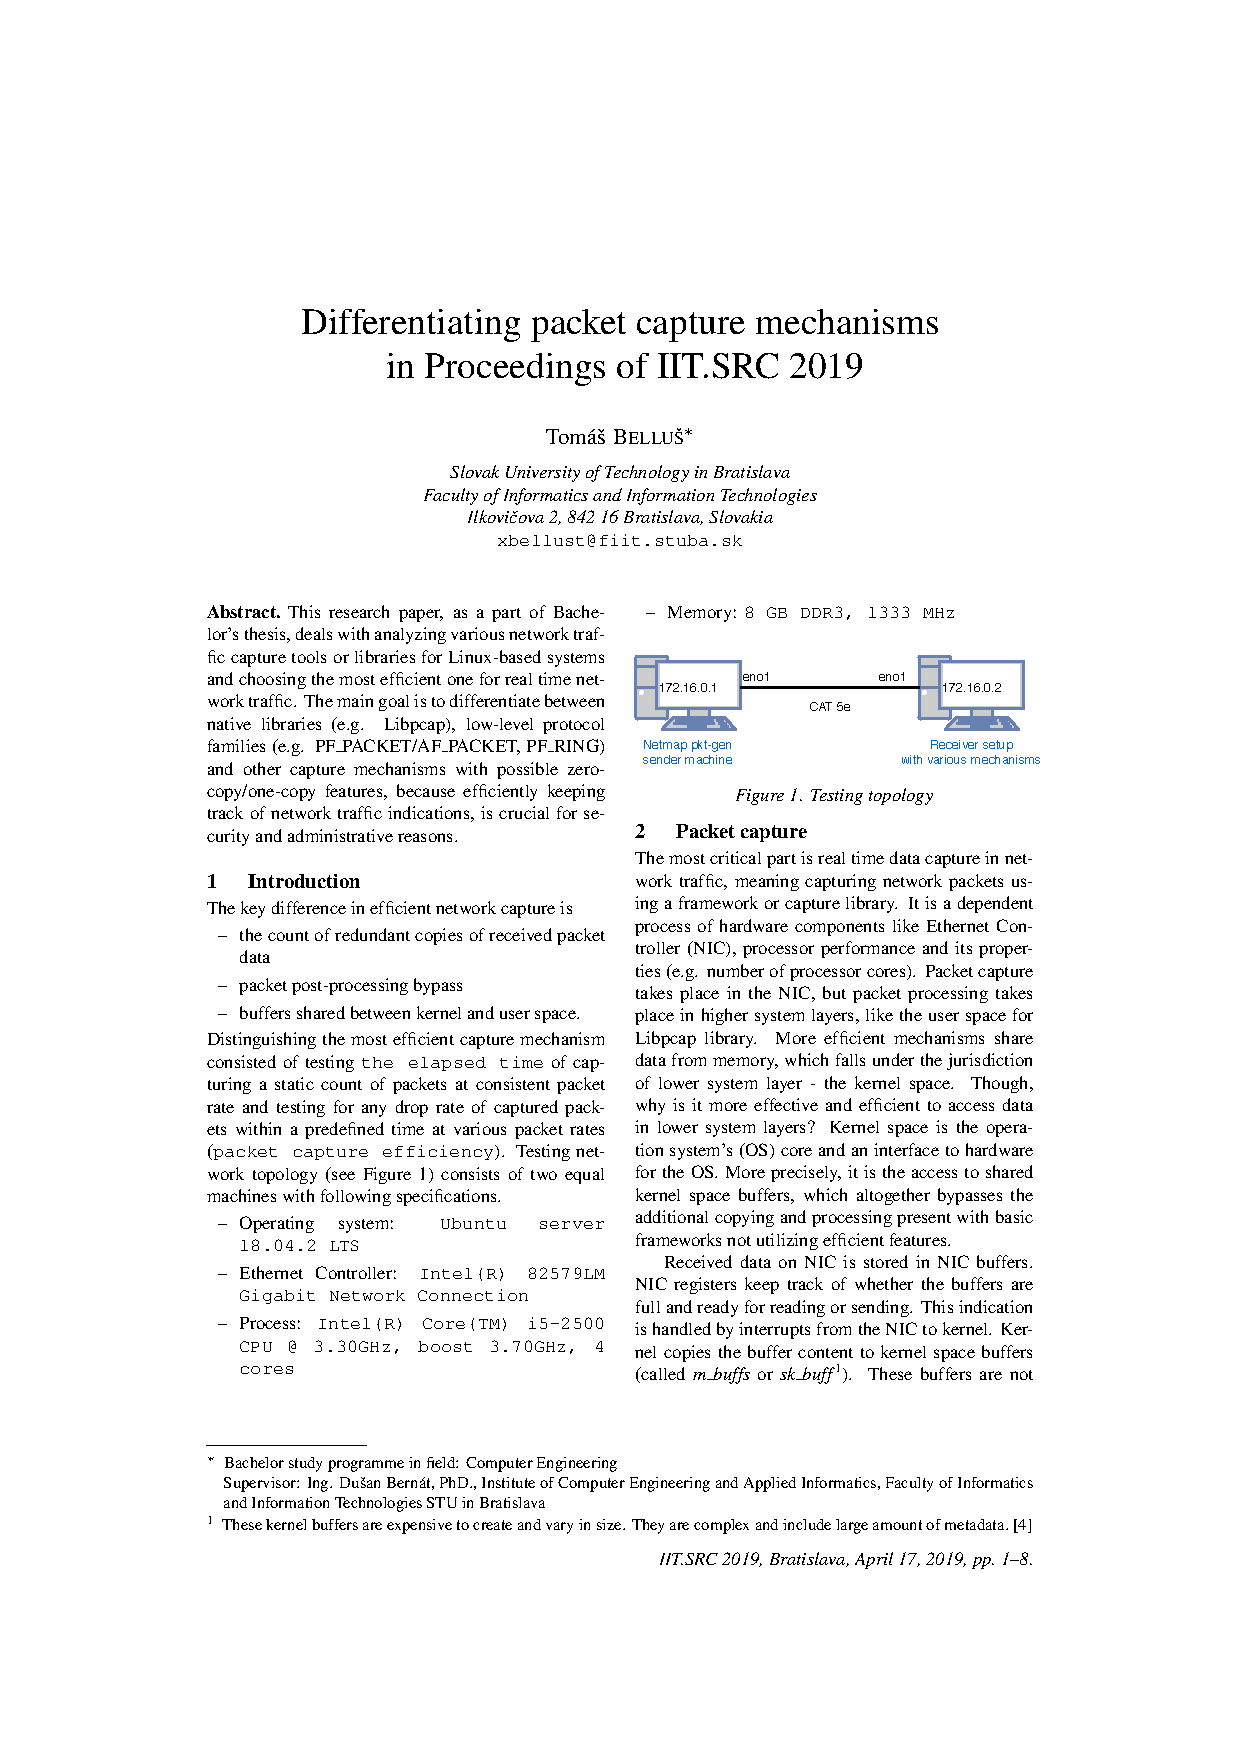
\includepdf[pages=-]{src/iitsrc_paper}
	\chapter{Kibana dashboard} \label{appendix:sol:dashboard}
		\begin{figure}[h]
			\centering
			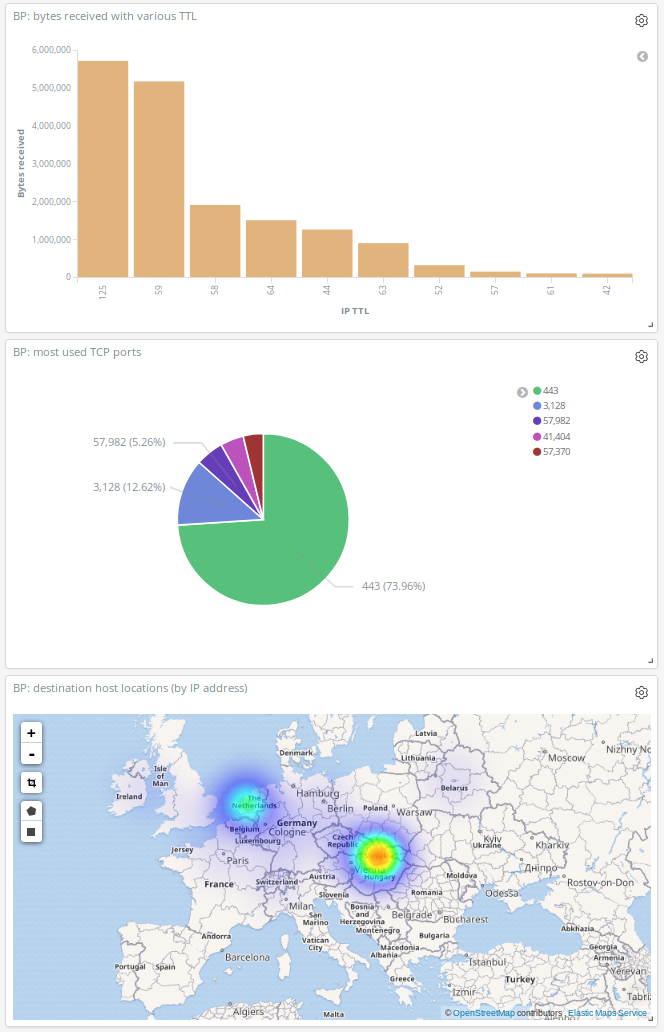
\includegraphics[scale=0.38]{dashboard}
		\end{figure}
	\chapter{Sensor configuration} \label{appendix:implementation:config}
		\lstinputlisting[language=bash, style=appendix, label=lst:sensor:config, caption=Configuration example]{src/config}
	\chapter{Logstash configuration} \label{appendix:implementation:logstash}
		\lstinputlisting[language=Clean, style=appendix]{src/logstash.conf}
	\chapter{Plan of work in winter semester}
		\lstinputlisting[language=Clean, style=appendix]{plan/december}	
	\chapter{Plan of work in summer semester}
		\lstinputlisting[language=Clean, style=appendix]{plan/may}
\end{appendices}
\end{document}
